\documentclass[11pt,a4paper,oneside,openany]{book}

\usepackage[T1]{fontenc}
\usepackage[italian]{babel}
\usepackage{amsmath,amssymb}
\usepackage[margin=2.5cm]{geometry}
\usepackage{graphicx}
\usepackage[ruled, lined, linesnumbered, algochapter]{algorithm2e}
\usepackage{listings}
\usepackage{tikz}
\usetikzlibrary{arrows.meta, positioning, shapes.geometric}
\renewcommand{\lstlistingname}{Struttura}

\renewcommand{\algorithmcfname}{Algoritmo}

\lstset{
    language=C,
    basicstyle=\ttfamily\small,
    keywordstyle=\bfseries,
    numbers=left,
    numberstyle=\bfseries\footnotesize,
    numbersep=10pt,
    frame=lines,
    framerule=0.8pt,
    captionpos=t,
    abovecaptionskip=4pt,
    belowcaptionskip=4pt,
    breaklines=true,
    showstringspaces=false
}

\newenvironment{listacomp}{%
    \small
    \begin{list}{\textendash}{%
        \setlength{\topsep}{2pt}%
        \setlength{\partopsep}{0pt}%
        \setlength{\itemsep}{1pt}%
        \setlength{\parsep}{0pt}%
        \setlength{\leftmargin}{1.2em}%
    }%
}{%
    \end{list}%
}

\begin{document}

\begin{titlepage}
\vspace*{1cm}
\begin{center}
{\LARGE\bfseries Report sistema di gestione Teatro \par}
\end{center}
\vspace*{10cm}

\noindent
\begin{minipage}[t]{0.65\textwidth}
\vspace{0pt}
{ \textbf{Nome e Cognome studente: } Renhao Chen \par}
\vspace*{0.2cm}
{ \textbf{Numero di matricola: } 130368 \par}
\vspace*{0.2cm}
{ \textbf{Anno accademico: } 2026/2027 \par}
\vspace*{0.2cm}
{ \textbf{Data di consegna: } \today \par}
\vspace*{0.2cm}
{ \textbf{Indirizzo github: } \par}
\end{minipage}
\hfill
\begin{minipage}[t]{0.3\textwidth}
    \vspace{0pt}
    \raggedleft
    
\includegraphics[width=3.5cm]{logo_unicam.png}
\end{minipage}


\vfill

\begin{flushleft}
\footnotesize
Documento scritto in \LaTeX.\\
Si fà riferimento per programma$ Chen_130368.c $pacchettato insieme. Per versione diverse guardare repository github.

\end{flushleft}
\end{titlepage}

\tableofcontents

\chapter{Introduzione}
\section{Problema da risolvere}
Il sistema è riferito per gestione di programmazione e prenotazioni dei biglietti di un Teatro Comunale.
Richiede di tenere traccia degli spettacoli in cartellone, dei clienti iscritti e delle prenotazioni effettuate.

\section{Obiettivi del progetto}
L'obiettivi del progetto sono:
- Verificare conoscenze sulle strutture di dati.
- Gestione della memoria e allocazione dinamica.
- Provare utilizzo dei nodi delle liste.
- Gestione File Binari / di Testo.
- Implementazione del codice in funzioni modularizzati.
- Passagio di parametri nelle funzioni in modalità sicure ed efficienti
- Gestione degli Errori.
- Interpretazione del Codice con commenti e Report.

\section{Tecnologie utilizzati}

Per lo sviluppo e la verifica del programma sono utilizatti i seguenti strumenti:
\begin{itemize}

\item \textbf{Linguaggio:} C (standard C11).
\item \textbf{Compilatore:} GCC (versione 16.1.0)
\item \textbf{Sistema operativo:}  Windows 10 (64-bit), Windows 11 Pro (64-bit)
\item \textbf{Ambiente di sviluppo:} Visual Studio Code.
\item \textbf{Controllo di versione:} Git e GitHub.
\end{itemize}

\chapter{Analisi del Problema}
\section{caso di studio}
Il programma deve essere comprensibile per operatore nella gestione degli atti, in due entità principali: Spettacoli (caraterizzati da codice spettacolo) in cartellone, Prenotazioni (caraterizzati da codice prenotazione) nelle liste effettuate dagli utenti

\section{Requisiti funzionali}
Il programma contiene seguenti funzionalità:
\begin{itemize}

    \item \textbf{Gestione del cartellone:} inserimento di nuovi spettacoli e clienti, ricerca con codice corrispondenti e visione in modo dettagliato dati inseriti ad ordine scelto.
    \item \textbf{Prenotazione e lista d'attesa:} registrazione delle prenotazioni fino ad esaurimento degli posti; in caso insuffuciente lasciare in lista d'attesa, e nel caso di annulazione prenotazione gestire correttamente lista d'attesa.
    \item \textbf{Scrittura e lettura dei dati presenti:} capacità di leggere dati già esistente nel file corrispondete, e nel caso contrario salvare dati presenti nel programma in file con formattazione giusto.
    \item \textbf{Calcoli statistici:} funzionalità di riassumere dati presenti in modo da comprendere situazione presenti e accomodare gestione in attesa.
\end{itemize}

\section{Requisiti non funzionali}
Oltre alle funzionalità principali, il sistema è stato progettato per rispettare i seguenti requisiti di non funzionali:
\begin{itemize}
\item \textbf{Performance:} utilizzo ottimizzato della memoria tramite allocazione dinamica e riallocazione neccessaria per garantire efficienza del programma.
\item \textbf{Usabilità:} interfaccia a riga di comando chiara e strutturata tramite in menu principali e vari menu secondarie distinti per funzionalità, con la richiesta di conferma per dati inseriti e messaggi di feedback espliciti.
\item \textbf{Robustezza:} controllo delle validità nel input, evitazione di blocchi infiniti, pulizia di buffer per utilizzo alternato di scanf e fgets.
\end{itemize}

\chapter{Progettazione}
\section{Struttre Dati}
\subsection{Struct utilizzati}
\begin{lstlisting}[caption={Definizione della struttura Spettacolo}]
typedef struct
{
    int codice_spettacolo;
    char titolo[101];
    char genere[31];
    char data_spettacolo[11];
    int posti_totali;
    int posti_disponibili;
    float prezzo_biglietto;
} Spettacolo;
\end{lstlisting}
Questa struttura di \texttt{Spettacolo} contiene:
\begin{listacomp}
    \item \textbf{Codice spettacolo:} codice univoco corrispondente allo spettacolo, inserito dall'utente e accettato effettivamente solo dopo averne verificato l'univocità.
    \item \textbf{Titolo:} stringa di lunghezza 101 considerando anche il carattere di fine stringa, che permette all'utente di inserire fino a 100 caratteri.
    \item \textbf{Genere:} stringa di lunghezza 31 considerando anche il carattere di fine stringa, che permette all'utente di inserire fino a 30 caratteri.
    \item \textbf{Data spettacolo:} stringa di formato \texttt{gg/mm/aaaa} fissato, validata dalle funzioni implementate.
    \item \textbf{Posti totali:} numero di tipo \texttt{int} strettamente positivo.
    \item \textbf{Posti disponibili:} numero di tipo \texttt{int} compreso tra 0 e i posti totali, inizializzato uguale a \texttt{posti\_totali}.
    \item \textbf{Prezzo biglietto:} numero di tipo \texttt{float} strettamente positivo.
\end{listacomp}

\begin{lstlisting}[caption={Definizione della struttura Cliente}]
typedef struct
{
    int codice_cliente;
    char nome[51];
    char cognome[51];
    char email[80];
    char data_iscrizione[11];
} Cliente;
\end{lstlisting}
Questa struttura di \texttt{Cliente} contiene:
\begin{listacomp}
    \item \textbf{Codice cliente:} codice univoco corrispondente al cliente, inserito dall'utente e accettato solo previa verifica di univocità.
    \item \textbf{Nome:} stringa di lunghezza 51 considerando anche il carattere di fine stringa, permettendo all'utente di inserire fino a 50 caratteri.
    \item \textbf{Cognome:} stringa di lunghezza 51 considerando anche il carattere di fine stringa, permettendo all'utente di inserire fino a 50 caratteri.
    \item \textbf{Email:} stringa di lunghezza 80 considerando anche il carattere di fine stringa (fino a 79 caratteri utili), validata tramite apposita funzione di controllo formale.
    \item \textbf{Data iscrizione:} stringa di lunghezza 11 nel formato \texttt{gg/mm/aaaa}, validata dalle funzioni implementate.
\end{listacomp}

\begin{lstlisting}[caption={Definizione della struttura Prenotazione}]
typedef struct
{
    int codice_prenotazione;
    int codice_spettacolo;
    int codice_cliente;
    int numero_posti;
    float importo_totale;
    char data_prenotazione[11];
} Prenotazione;
\end{lstlisting}
Questa struttura di \texttt{Prenotazione} contiene:
\begin{listacomp}
    \item \textbf{Codice prenotazione:} chiave univoca di tipo \texttt{int} generata automaticamente in modo incrementale dal sistema.
    \item \textbf{Codice spettacolo:} identificativo numerico che collega la prenotazione allo spettacolo selezionato.
    \item \textbf{Codice cliente:} identificativo numerico che collega la prenotazione al cliente richiedente.
    \item \textbf{Numero posti:} numero di tipo \texttt{int} corrispondente ai biglietti prenotati (compreso tra 1 e un massimo di 10 per singola prenotazione).
    \item \textbf{Importo totale:} numero di tipo \texttt{float} calcolato automaticamente moltiplicando il numero di posti prenotati per il prezzo unitario del biglietto dello spettacolo.
    \item \textbf{Data prenotazione:} stringa di lunghezza 11 nel formato \texttt{gg/mm/aaaa}, validata dalle funzioni implementate.
\end{listacomp}

\begin{lstlisting}[caption={Definizione della struttura RichiestaAttesa}]
typedef struct
{
    int codice_spettacolo;
    int codice_cliente;
    int numero_posti;
    char data_richiesta[11];
} RichiestaAttesa;
\end{lstlisting}
Questa struttura di \texttt{RichiestaAttesa} contiene:
\begin{listacomp}
    \item \textbf{Codice spettacolo:} codice univoco dello spettacolo per cui il cliente viene inserito in lista d'attesa.
    \item \textbf{Codice cliente:} codice univoco del cliente che ha effettuato la richiesta in assenza di posti disponibili.
    \item \textbf{Numero posti:} numero di tipo \texttt{int} che indica i biglietti richiesti, con limite massimo predefinito pari a 10.
    \item \textbf{Data richiesta:} stringa di lunghezza 11 nel formato \texttt{gg/mm/aaaa} che registra la data di inserimento in coda.
\end{listacomp}

\begin{lstlisting}[caption={Definizione della struttura NodoPrenotazione}]
typedef struct NodoPrenotazione
{
    Prenotazione dati;
    struct NodoPrenotazione *next;
} NodoPrenotazione;
\end{lstlisting}
Questa struttura di \texttt{NodoPrenotazione} rappresenta il singolo elemento della lista concatenata delle prenotazioni e contiene:
\begin{listacomp}
    \item \textbf{Dati:} struttura di tipo \texttt{Prenotazione} contenente tutte le informazioni relative alla singola prenotazione.
    \item \textbf{Next:} puntatore al nodo successivo della lista concatenata (oppure \texttt{NULL} se il nodo è l'ultimo della lista).
\end{listacomp}

\begin{lstlisting}[caption={Definizione della struttura NodoAttesa}]
typedef struct NodoAttesa
{
    RichiestaAttesa dati;
    struct NodoAttesa *next;
} NodoAttesa;
\end{lstlisting}
Questa struttura di \texttt{NodoAttesa} rappresenta il singolo elemento della lista concatenata d'attesa (gestita in modalità FIFO) e contiene:
\begin{listacomp}
    \item \textbf{Dati:} struttura di tipo \texttt{RichiestaAttesa} contenente i dettagli della richiesta in coda.
    \item \textbf{Next:} puntatore al nodo successivo nella coda d'attesa (oppure \texttt{NULL} in corrispondenza dell'ultimo elemento).
\end{listacomp}

\begin{lstlisting}[caption={Definizione della struttura Nodogenere}]
typedef struct Nodogenere
{
    char genere[51];
    int numero;
    struct Nodogenere *next;
} Nodogenere;
\end{lstlisting}
Questa struttura di \texttt{Nodogenere} costituisce il nodo di una lista dinamica di appoggio utilizzata per il calcolo delle statistiche per genere e contiene:
\begin{listacomp}
    \item \textbf{Genere:} stringa di lunghezza 51 considerando anche il carattere di fine stringa (fino a 50 caratteri utili), che memorizza il nome del genere teatrale analizzato.
    \item \textbf{Numero:} contatore di tipo \texttt{int} che accumula il totale delle occorrenze o delle prenotazioni associate a quel determinato genere.
    \item \textbf{Next:} puntatore al nodo successivo della lista statistica.
\end{listacomp}

\subsection{Motivazione delle scelte progettuali}
L'architettura del programma è stata progettata bilanciando efficienza nell'accesso ai dati, flessibilità nella gestione della memoria dinamica e modularità del codice. Le principali scelte implementative sono le seguenti:

\begin{listacomp}
    \item \textbf{Uso combinato di array dinamici e liste concatenate:} per le entità \texttt{Spettacolo} e \texttt{Cliente} sono stati adottati array allocati dinamicamente (ridimensionati tramite \texttt{realloc}), poiché tali strutture richiedono frequenti operazioni di ricerca e ordinamento (come l'ordinamento degli spettacoli per posti disponibili). Al contrario, per \texttt{NodoPrenotazione} e \texttt{NodoAttesa} si è optato per liste concatenate, così da gestire inserimenti e cancellazioni frequenti senza il costo computazionale dello scorrimento degli elementi in memoria.
    \item \textbf{Gestione FIFO della lista d'attesa:} la lista d'attesa è stata implementata secondo una politica \emph{First-In, First-Out} (inserimento in coda ed estrazione in testa). Questa scelta garantisce l'assegnazione equa e cronologica dei biglietti nel momento in cui una prenotazione precedente viene annullata.
    \item \textbf{Lista dinamica di appoggio per le statistiche:} per il calcolo delle statistiche per genere è stata introdotta la struttura \texttt{Nodogenere}, che permette di aggregare i dati dinamicamente senza dover fissare a priori un numero massimo di generi teatrali.
    \item \textbf{Separazione delle operazioni di I/O e tolleranza all'avvio:} il caricamento e il salvataggio su file sono stati separati in funzioni distinte per mantenere sincronizzati gli archivi ed evitare letture o sovrascritture ridondanti. Inoltre, l'assenza dei file al primo avvio non provoca l'arresto del programma, ma inizializza correttamente le strutture vuote.
    \item \textbf{Modularizzazione e validazione centralizzata:} le verifiche su formato delle date (\texttt{gg/mm/aaaa}), validità degli indirizzi email, univocità dei codici identificativi e pulizia del buffer di input sono state isolate in funzioni ausiliarie riutilizzabili, evitando duplicazioni di codice e garantendo l'integrità dei dati in memoria.
\end{listacomp}

\subsection{{Diagramma}}

\begin{figure}[htbp]
\centering
\begin{tikzpicture}[
    font=\footnotesize,
    struttura/.style={
        draw=black!85,
        thick,
        rounded corners=2pt,
        align=left,
        fill=gray!6,
        inner sep=6pt
    },
    funzione/.style={
        draw=black!85,
        thick,
        rounded corners=5pt,
        align=center,
        fill=gray!16,
        inner sep=5pt
    },
    freccia/.style={-{Stealth[length=2.2mm]}, thick, draw=black!85}
]

% FASCIA 1 (Alto): Strutture principali (Array Dinamici)
\node[struttura, text width=5.0cm] (spettacolo) at (-4.2, 0) {
    \centering\textbf{\small Spettacolo} \scriptsize(Array Dinamico)\par\vspace{2pt}\hrule\vspace{3pt}
    \raggedright
    \underline{\textbf{codice\_spettacolo}} \scriptsize(univoco)\footnotesize\\
    titolo, genere, data\_spettacolo\\
    posti\_totali, posti\_disponibili\\
    prezzo\_biglietto
};

\node[struttura, text width=5.0cm] (cliente) at (4.2, 0) {
    \centering\textbf{\small Cliente} \scriptsize(Array Dinamico)\par\vspace{2pt}\hrule\vspace{3pt}
    \raggedright
    \underline{\textbf{codice\_cliente}} \scriptsize(univoco)\footnotesize\\
    nome, cognome\\
    email\\
    data\_iscrizione
};

% Raccordo superiore (tra Fascia 1 e Fascia 2)
\draw[thick] (spettacolo.south) -- (-4.2, -1.95);
\draw[thick] (cliente.south) -- (4.2, -1.95);
\draw[thick] (-5.3, -1.95) -- (5.3, -1.95);

% FASCIA 2 (Centro): Funzioni di collegamento e controllo
\node[funzione, text width=3.5cm, minimum height=1.35cm] (fn_sp) at (-5.3, -3.65) {
    \textbf{Ricerca Spettacolo}\\
    \scriptsize\texttt{controllacodiceSp()}
};

\node[funzione, text width=4.5cm, minimum height=1.35cm] (fn_mid) at (0, -3.65) {
    \textbf{Gestione Prenotazioni e Attese}\\
    \scriptsize\texttt{registraprenotazione()}\\
    \texttt{annullaprenotazione()}\\
    \texttt{converteprenotazione()}
};

\node[funzione, text width=3.5cm, minimum height=1.35cm] (fn_cl) at (5.3, -3.65) {
    \textbf{Ricerca e Report Clienti}\\
    \scriptsize\texttt{controllacodiceCl()}\\
    \texttt{esportaprenotazione()}
};

\draw[freccia] (-5.3, -1.95) -- (fn_sp.north);
\draw[freccia] (0, -1.95) -- (fn_mid.north);
\draw[freccia] (5.3, -1.95) -- (fn_cl.north);

% Raccordo inferiore (tra Fascia 2 e Fascia 3)
\draw[thick] (fn_sp.south) -- (-5.3, -5.45);
\draw[thick] (fn_mid.south) -- (0, -5.45);
\draw[thick] (fn_cl.south) -- (5.3, -5.45);
\draw[thick] (-5.3, -5.45) -- (5.3, -5.45);

% FASCIA 3 (Basso): Strutture associative (Liste Concatenate)
\node[struttura, text width=5.2cm] (prenotazione) at (-4.2, -7.2) {
    \centering\textbf{\small Prenotazione} \scriptsize(Lista Concatenata)\par\vspace{2pt}\hrule\vspace{3pt}
    \raggedright
    \underline{\textbf{codice\_prenotazione}} \scriptsize(univoco)\footnotesize\\
    \textit{codice\_spettacolo}, \textit{codice\_cliente}\\
    numero\_posti, importo\_totale\\
    data\_prenotazione
};

\node[struttura, text width=5.2cm] (attesa) at (4.2, -7.2) {
    \centering\textbf{\small RichiestaAttesa} \scriptsize(Lista Concatenata)\par\vspace{2pt}\hrule\vspace{3pt}
    \raggedright
    \textit{codice\_spettacolo}, \textit{codice\_cliente}\\
    numero\_posti\\
    data\_richiesta
};

\draw[freccia] (-4.2, -5.45) -- (prenotazione.north);
\draw[freccia] (4.2, -5.45) -- (attesa.north);

\end{tikzpicture}
\caption{Collegamento tra le strutture dati tramite codici e funzioni di gestione.}
\label{fig:relazioni_funzioni_tikz}
\end{figure}

Come illustrato in Figura~\ref{fig:relazioni_funzioni_tikz}, l'organizzazione dei dati su tre livelli consente di collegare le entità principali del teatro alle operazioni operative tramite i rispettivi codici identificativi:
\begin{listacomp}
    \item \textbf{Strutture principali (fascia superiore):} gli array dinamici \texttt{Spettacolo} e \texttt{Cliente} conservano i dati anagrafici e sono identificati univocamente tramite i campi \texttt{codice\_spettacolo} e \texttt{codice\_cliente}.
    \item \textbf{Strutture di collegamento (fascia inferiore):} le liste concatenate \texttt{Prenotazione} e \texttt{RichiestaAttesa} associano un cliente a uno spettacolo memorizzando esclusivamente i riferimenti \texttt{codice\_spettacolo} e \texttt{codice\_cliente}, evitando la duplicazione di titoli, prezzi o dati personali in memoria.
    \item \textbf{Ricerca e validazione (\texttt{controllacodiceSp} e \texttt{controllacodiceCl}):} scorrono rispettivamente gli array \texttt{Spettacolo} e \texttt{Cliente} per verificare l'univocità dei codici in fase di inserimento e per ricavare l'indice dell'elemento corrispondente durante le operazioni di prenotazione, annullamento ed esportazione.
    \item \textbf{Flusso prenotazioni e subentro (\texttt{registraprenotazione}, \texttt{annullaprenotazione} e \texttt{converteprenotazione}):} gestiscono l'interazione tra gli array e le due liste concatenate; in particolare, aggiornano \texttt{posti\_disponibili} nell'array \texttt{Spettacolo}, calcolano \texttt{importo\_totale} tramite \texttt{prezzo\_biglietto} e, in caso di annullamento, convertono automaticamente le richieste compatibili da \texttt{RichiestaAttesa} a \texttt{Prenotazione}.
    \item \textbf{Incrocio dati per reportistica (\texttt{esportaprenotazione}):} utilizza il campo \texttt{codice\_cliente} presente in ogni nodo di \texttt{Prenotazione} per risalire a nome e cognome nell'array \texttt{Cliente} e generare il riepilogo testuale in \texttt{report\_prenotazioni.txt}.
\end{listacomp}

\section{Architettura del sistema}
\subsection{Descrizione dell'organizzazione del codice}
Il Codice è strutturato in modo seguente:
\begin{listacomp}
\item \textbf{Inclusione di libreria neccessaria:} includo librerie come <stdio.h> come base, <stdlib.h> per allocazione dinamica, <string.h> per gestione di stringhe
\item \textbf{definizione di strutture:} Inizio a definire tutte le strutture che viene richiesto contenente pure i nodi delle liste.
\item \textbf{dichiarazione di funzioni prototipo:} tutte le funzione utilizzate vengono dichiarati in quasta parte in maniera prototipo, con specificazioni commentati e raggrupate in base alle funzionalità svolte e caratteristiche.
\item \textbf{main:} parte minimizzata, richiama prima funzione avvio(), in richiesta di inserire password con defaul 123456 per entrare in programma, tutte le operazione vengono effettuati dentro funzione menu, e utlima riga il return 0.
\item \textbf{implementazione delle funzioni:} tutte le funzioni vengono scritti secondo ordine di dichiarazione, ovvero tutti ordinati e distinti in base alla funzionalità.
\end{listacomp}

\subsection{Elenco delle funzioni principali con breve descrizione}
Le funzioni principali implementate in \texttt{$Chen_130368.c$} sono:
\begin{listacomp}
    \item \textbf{\texttt{avvio ()}:} gestisce l'accesso al sistema richiedendo la password salvata in \texttt{password.dat} (impostata a \texttt{123456} come valore predefinito) e consentendo eventualmente di modificarla prima di entrare nel menu.
    \item \textbf{\texttt{menu ()}:} inizializza gli array dinamici e le liste concatenate, gestisce il ciclo principale di smistamento verso i sottomenu e, in fase di uscita, richiama \texttt{liberazione()} per deallocare tutta la memoria dinamica.
    \item \textbf{\texttt{inserimentospettacolo ()}:} acquisisce da tastiera i dati di un nuovo spettacolo, ne verifica l'univocità del codice e la validità formale, e richiede conferma finale prima della registrazione nell'array.
    \item \textbf{\texttt{riallocazioneSp ()}:} confronta il numero di spettacoli inseriti con la capacità massima allocata e ridimensiona dinamicamente l'array tramite \texttt{realloc} (in modo automatico o su dimensione specificata dall'utente).
    \item \textbf{\texttt{converteprenotazione ()}:} ripristina i posti liberati dopo l'annullamento di una prenotazione e scorre la lista d'attesa convertendo automaticamente in prenotazioni attive le richieste compatibili con i posti disponibili.
    \item \textbf{\texttt{caricadatabase ()}:} legge gli archivi binari (\texttt{.dat}), adegua la capacità degli array dinamici, libera le liste preesistenti e carica in memoria i dati aggiornati ricostruendo anche la lista dei generi.
\end{listacomp}

\subsection{Schema del flusso del programma}

\begin{figure}[htbp]
\centering
\begin{tikzpicture}[
    font=\footnotesize,
    terminale/.style={
        draw=black!85,
        thick,
        rounded corners=8pt,
        align=center,
        fill=gray!16,
        inner sep=5pt
    },
    processo/.style={
        draw=black!85,
        thick,
        rounded corners=2pt,
        align=center,
        fill=gray!6,
        inner sep=5pt
    },
    sottomenu/.style={
        draw=black!85,
        thick,
        rounded corners=2pt,
        align=center,
        fill=gray!8,
        inner sep=4pt
    },
    decisione/.style={
        diamond,
        aspect=2.3,
        draw=black!85,
        thick,
        align=center,
        fill=gray!12,
        inner sep=3pt
    },
    freccia/.style={-{Stealth[length=2.2mm]}, thick, draw=black!85}
]

% 1. Avvio e inizializzazione
\node[terminale, text width=9.2cm] (start) at (0, 0) {
    \textbf{Inizio (\texttt{main()}) -- Autenticazione (\texttt{avvio()})}\\
    Verifica password e allocazione array dinamici
};

% 2. Ciclo Menu Principale
\node[processo, text width=6.6cm] (menu) at (0, -2.1) {
    \textbf{Ciclo Menu Principale (\texttt{menu()})}\\
    Lettura scelta utente (opzioni A--F)
};

\draw[freccia] (start.south) -- (menu.north);

% 3. Diramazione verso i 5 Menu Secondari (A-E)
\draw[thick] (menu.south) -- (0, -3.15);
\node[right] at (0.1, -2.88) {Scelte A--E};
\draw[thick] (-5.4, -3.15) -- (5.4, -3.15);

\node[sottomenu, text width=2.15cm] (mA) at (-5.4, -4.35) {
    \textbf{A. Spettacoli}\\
    \texttt{menuspettacoli}\\
    Ciclo interno
};

\node[sottomenu, text width=2.15cm] (mB) at (-2.7, -4.35) {
    \textbf{B. Clienti}\\
    \texttt{menuclienti}\\
    Ciclo interno
};

\node[sottomenu, text width=2.15cm] (mC) at (0, -4.35) {
    \textbf{C. Prenotazioni}\\
    \texttt{menuprenotazioni}\\
    Ciclo interno
};

\node[sottomenu, text width=2.15cm] (mD) at (2.7, -4.35) {
    \textbf{D. Statistiche}\\
    \texttt{menustat}\\
    Ciclo interno
};

\node[sottomenu, text width=2.15cm] (mE) at (5.4, -4.35) {
    \textbf{E. Gestione File}\\
    \texttt{menufile}\\
    Ciclo interno
};

\foreach \x/\nodo in {-5.4/mA, -2.7/mB, 0/mC, 2.7/mD, 5.4/mE} {
    \draw[freccia] (\x, -3.15) -- (\nodo.north);
    \draw[thick] (\nodo.south) -- (\x, -6.05);
}

% Linea di raccolta e ritorno dai 5 sottomenu (ben distanziata sotto i riquadri)
\draw[thick] (5.4, -6.05) -- (-7.35, -6.05);
\node[above] at (-2.7, -6.02) {Uscita dal sottomenu (ritorno al menu principale)};
\draw[freccia] (-7.35, -6.05) -- (-7.35, -1.15) -- (0, -1.15);

% 4. Ramo F (Uscita) lungo il corridoio destro
\draw[thick] (menu.east) -- (7.35, -2.1);
\node[above] at (5.35, -2.07) {Scelta F (Esci)};
\draw[freccia] (7.35, -2.1) -- (7.35, -6.7) -- (0, -6.7) -- (0, -7.05);

% 5. Decisione Conferma Uscita
\node[decisione] (exit_dec) at (0, -7.8) {
    \textbf{Conferma}\\
    \textbf{uscita?}
};

% Opzione 3: Non uscire (rientra nel corridoio sinistro dentro i margini)
\draw[thick] (exit_dec.west) -- (-7.35, -7.8);
\node[above] at (-4.65, -7.77) {3: Non uscire (ritorna)};
\draw[thick] (-7.35, -7.8) -- (-7.35, -6.05);

% Opzione 2: Salva ed esci
\node[processo, text width=4.0cm] (salva) at (4.6, -9.15) {
    \textbf{Salvataggio dati}\\
    \texttt{salvadatabase()}
};
\draw[freccia] (exit_dec.east) -| (salva.north)
    node[pos=0.28, above] {2: Salva};

% Opzione 1: Esci direttamente + Liberazione memoria
\node[processo, text width=8.6cm] (libera) at (0, -10.95) {
    \textbf{Liberazione della memoria (\texttt{liberazione()})}\\
    Deallocazione array dinamici e liste concatenate
};

\node[terminale, text width=3.8cm] (fine) at (0, -12.45) {
    \textbf{Fine Programma}
};

\draw[freccia] (exit_dec.south) -- (libera.north)
    node[pos=0.30, left] {1: Diretto};
\draw[freccia] (salva.south) |- (0, -10.05);
\draw[freccia] (libera.south) -- (fine.north);

\end{tikzpicture}
\caption{Diagramma di flusso del programma con diramazione dei 5 menu secondari e gestione dell'uscita.}
\label{fig:flusso_programma}
\end{figure}

\section{Gestione della memoria}
\subsection{Allocazione dinamica degli array}
All'avvio della funzione \texttt{menu()}, il programma richiede all'utente due interi strettamente positivi tramite \texttt{richiestaMaxspettacoli()} e \texttt{richiestaMaxclienti()}, che definiscono le capacità iniziali degli array per gli spettacoli e i clienti. Lo spazio viene quindi riservato sullo \emph{heap} mediante le funzioni dedicate \texttt{avviospettacoli()} e \texttt{avvioclienti()}, le quali incapsulano la chiamata a \texttt{malloc()} e verificano che il puntatore restituito non sia \texttt{NULL}. Prima e dopo ogni nuovo inserimento (\texttt{inserimentospettacolo()} e \texttt{inserimentoclienti()}), la funzione \texttt{controllospazio()} confronta il numero di elementi presenti con la capacità massima attuale e, se necessario, attiva \texttt{riallocazioneSp()} o \texttt{riallocazioneCl()} per espandere la memoria tramite \texttt{realloc()}. Gli stessi controlli di capienza e riallocazione vengono eseguiti anche in \texttt{caricadatabase()} prima di leggere i record dai file binari, evitando qualsiasi scrittura oltre i limiti allocati.

\subsection{Deallocazione}
La strategia di rilascio della memoria distingue tra strutture contigue e strutture concatenate:
\begin{listacomp}
    \item \textbf{Array dinamici:} fatta eccezione per gli eventuali ridimensionamenti intermedi gestiti da \texttt{realloc()}, gli array \texttt{Spettacoli} e \texttt{Clienti} restano allocati per l'intera durata dell'esecuzione e vengono liberati unicamente alla chiusura del programma tramite \texttt{free()} all'interno della funzione \texttt{liberazione()}. Fanno eccezione gli array di appoggio \texttt{incassi} e \texttt{indici} utilizzati in \texttt{stampatop()} e \texttt{spettacolidisponibili()}, che vengono deallocati localmente al termine della rispettiva funzione.
    \item \textbf{Liste concatenate:} oltre alla deallocazione completa effettuata alla chiusura del programma (tramite \texttt{liberaprenotazioni()}, \texttt{liberaattesa()} e \texttt{liberageneri()}, che scorrono ciascuna lista liberando ogni nodo attraversato), i singoli nodi possono essere rilasciati anche a \emph{runtime}. Ciò avviene quando si annulla una prenotazione (\texttt{Eliminaprenotazione()}), quando una richiesta in attesa viene convertita in prenotazione attiva (\texttt{converteprenotazione()}) oppure prima di ricaricare gli archivi da file (\texttt{caricadatabase()}).
\end{listacomp}

\subsection{Ciclo di vita delle strutture dati}
Gli array dinamici vengono creati all'inizio della sessione in \texttt{menu()}, subito dopo l'acquisizione delle dimensioni iniziali. Le liste concatenate delle prenotazioni, delle richieste d'attesa e dei generi vengono invece inizializzate a \texttt{NULL} (liste vuote): un nuovo nodo viene allocato (\texttt{creaprenotazione()} o \texttt{creaattesa()}) e inserito in coda (\texttt{inserimentocodaprenotazione()} o \texttt{inserimentocodaattesa()}) solo dopo che l'utente ha confermato i dati inseriti, aggiornando il puntatore di testa quando necessario. Un comportamento specifico riguarda la lista \texttt{Nodogenere}: a ogni inserimento valido di uno spettacolo, la funzione \texttt{valutagenere()} verifica se il genere è già presente nella lista; in caso affermativo incrementa il relativo contatore \texttt{numero}, altrimenti crea e accoda un nuovo nodo con contatore inizializzato a \texttt{1}.

Durante il caricamento da file (\texttt{caricadatabase()}), una volta verificata l'apertura e la lettura dell'intestazione di \texttt{spettacoli.dat}, i contatori \texttt{num\_spettacoli} e \texttt{num\_clienti} vengono azzerati in modo da sovrascrivere gli array esistenti, mentre le liste concatenate precedenti vengono interamente deallocate e ricostruite nodo per nodo a partire dai dati letti dai file binari. Al termine dell'esecuzione, tutta la memoria dinamica residua viene liberata prima dell'uscita.

\subsection{Zone di memoria coinvolte}
Nel corso dell'esecuzione, le variabili e le strutture dati del programma sono distribuite tra \emph{stack} e \emph{heap} secondo il loro ciclo di vita:
\begin{listacomp}
    \item \textbf{Memoria \emph{Stack}:} ospita i record di attivazione delle funzioni, i parametri passati per valore o per indirizzo e tutte le variabili locali con dimensione nota a tempo di compilazione. Rientrano in questa area i contatori e le capacità (\texttt{num\_spettacoli}, \texttt{num\_clienti}, \texttt{Maxspettacoli}, \texttt{Maxclienti}), le variabili di controllo dei menu (\texttt{primascelta}, \texttt{secondascelta}), gli indici dei cicli, i puntatori ai file (\texttt{FILE *fp}), le strutture temporanee d'appoggio (come \texttt{Prenotazione dati} o \texttt{RichiestaAttesa datiattesa}), i buffer locali per la validazione delle stringhe (\texttt{tempdata[11]}, \texttt{tempemail[81]}, \texttt{genere[31]}) nonché le variabili puntatore stesse (\texttt{Spettacoli}, \texttt{Clienti}, \texttt{Prenotazioni}, \texttt{Attese}, \texttt{generi}). Tali dati vengono allocati automaticamente all'ingresso della funzione e rimossi al suo ritorno.
    \item \textbf{Memoria \emph{Heap}:} ospita tutti i blocchi allocati dinamicamente a \emph{runtime} tramite \texttt{malloc ()} e \texttt{realloc ()}, 
    la cui durata non è legata allo scope della singola funzione ma è gestita esplicitamente dal programmatore tramite puntatori e chiamate a \texttt{free ()}. 
    Appartengono allo \emph{heap} i due array contigui di strutture \texttt{Spettacolo} e \texttt{Cliente}, tutti i nodi delle liste concatenate (\texttt{NodoPrenotazione}, \texttt{NodoAttesa} e \texttt{Nodogenere}) e gli array ausiliari dinamici (\texttt{incassi} e \texttt{indici}) allocati temporaneamente per le operazioni di ordinamento.
\end{listacomp}

\section{Gestione delle Liste}

\subsection{Motivazione}
Per memorizzare le prenotazioni attive e le richieste in lista d'attesa sono state adottate liste concatenate semplici (\texttt{NodoPrenotazione} e \texttt{NodoAttesa}), in cui ciascun elemento è composto da una struttura dati informativa (\texttt{dati}) e da un puntatore (\texttt{next}) all'elemento successivo.

Questa scelta offre due vantaggi principali rispetto agli array: consente di inserire nuovi elementi dinamicamente senza dover stimare a priori la dimensione massima della struttura, e permette di rimuovere un nodo in qualsiasi posizione modificando esclusivamente i puntatori adiacenti, preservando l'ordine cronologico senza dover traslare gli elementi successivi in memoria. Di contro, poiché l'indirizzo di ogni nodo è conservato unicamente nel nodo che lo precede, non è possibile l'accesso diretto tramite indice: ogni operazione di ricerca richiede lo scorrimento sequenziale a partire dalla testa della lista, e l'eventuale perdita del puntatore di testa comporterebbe l'impossibilità di raggiungere e deallocare l'intera struttura.

\subsection{Schema grafico}
La Figura~\ref{fig:schema_lista} rappresenta la struttura logica in memoria di una lista concatenata utilizzata nel programma: il puntatore di testa mantiene il riferimento al primo nodo, mentre ciascun nodo collega la propria sezione dati al nodo successivo fino al terminatore \texttt{NULL}.

\begin{figure}[htbp]
\centering
\begin{tikzpicture}[
    font=\footnotesize,
    freccia/.style={-{Stealth[length=2.2mm]}, thick, draw=black!85}
]

% Puntatore di testa
\draw[thick, fill=gray!14, rounded corners=2pt] (-6.3, -0.45) rectangle (-4.3, 0.45);
\node[align=center] at (-5.3, 0) {\textbf{Testa}\\ \texttt{Prenotazioni}};

\draw[freccia] (-4.3, 0) -- (-3.3, 0);

% Nodo 1
\draw[thick, fill=gray!6] (-3.3, -0.45) rectangle (-1.7, 0.45);
\draw[thick, fill=gray!12] (-1.7, -0.45) rectangle (-0.8, 0.45);
\node at (-2.5, 0) {\texttt{dati}};
\node at (-1.25, 0) {\texttt{next}};
\node[below] at (-2.05, -0.55) {Nodo 1};

\draw[freccia] (-0.8, 0) -- (0.3, 0);

% Nodo 2
\draw[thick, fill=gray!6] (0.3, -0.45) rectangle (1.9, 0.45);
\draw[thick, fill=gray!12] (1.9, -0.45) rectangle (2.8, 0.45);
\node at (1.1, 0) {\texttt{dati}};
\node at (2.35, 0) {\texttt{next}};
\node[below] at (1.55, -0.55) {Nodo 2};

\draw[freccia] (2.8, 0) -- (3.9, 0);

% NULL
\draw[thick, fill=gray!14, rounded corners=2pt] (3.9, -0.35) rectangle (5.1, 0.35);
\node at (4.5, 0) {\texttt{NULL}};

\end{tikzpicture}
\caption{Rappresentazione grafica della struttura di una lista concatenata.}
\label{fig:schema_lista}
\end{figure}

\subsection{Algoritmo di inserimento in coda}
L'inserimento in coda viene utilizzato sia per registrare le nuove prenotazioni in ordine cronologico sia per garantire la politica FIFO (\emph{First-In, First-Out}) nella lista d'attesa. Come mostrato in Figura~\ref{fig:inserimento_coda}, un puntatore ausiliario \texttt{p} scorre la lista fino all'ultimo nodo (\texttt{p->next == NULL}) e aggancia il nuovo elemento aggiornando i puntatori.

\begin{figure}[htbp]
\centering
\begin{tikzpicture}[
    font=\footnotesize,
    freccia/.style={-{Stealth[length=2.2mm]}, thick, draw=black!85}
]

% Testa
\draw[thick, fill=gray!14, rounded corners=2pt] (-6.3, -0.4) rectangle (-4.6, 0.4);
\node at (-5.45, 0) {\textbf{Testa}};
\draw[freccia] (-4.6, 0) -- (-3.6, 0);

% Nodo 1
\draw[thick, fill=gray!6] (-3.6, -0.4) rectangle (-2.2, 0.4);
\draw[thick, fill=gray!12] (-2.2, -0.4) rectangle (-1.4, 0.4);
\node at (-2.9, 0) {\texttt{dati}};
\node at (-1.8, 0) {\texttt{next}};
\draw[freccia] (-1.4, 0) -- (-0.3, 0);

% Nodo 2 (ultimo nodo corrente)
\draw[thick, fill=gray!6] (-0.3, -0.4) rectangle (1.1, 0.4);
\draw[thick, fill=gray!12] (1.1, -0.4) rectangle (1.9, 0.4);
\node at (0.4, 0) {\texttt{dati}};
\node at (1.5, 0) {\texttt{next}};

% Puntatore p
\node[above] at (0.8, 1.0) {\texttt{p} (\texttt{p->next == NULL})};
\draw[freccia] (0.8, 1.0) -- (0.8, 0.45);

% Vecchio collegamento a NULL
\draw[freccia, dashed] (1.9, 0) -- (3.1, 0);
\draw[thick, dashed, rounded corners=2pt] (3.1, -0.35) rectangle (4.3, 0.35);
\node at (3.7, 0) {\texttt{NULL}};

% Nuovo nodo in basso
\draw[thick, fill=gray!16] (2.1, -2.2) rectangle (3.5, -1.4);
\draw[thick, fill=gray!22] (3.5, -2.2) rectangle (4.3, -1.4);
\node at (2.8, -1.8) {\texttt{dati}};
\node at (3.9, -1.8) {\texttt{next}};
\node[below] at (3.2, -2.3) {Nuovo nodo};

% Collegamenti nuovi
\draw[freccia] (1.5, -0.4) |- (2.1, -1.8);
\node[left] at (1.45, -1.25) {\textbf{1.} \texttt{p->next = nuovo}};

\draw[freccia] (4.3, -1.8) -- (5.3, -1.8);
\draw[thick, fill=gray!14, rounded corners=2pt] (5.3, -2.15) rectangle (6.5, -1.45);
\node at (5.9, -1.8) {\texttt{NULL}};
\node[above] at (4.85, -1.45) {\textbf{2.}};

\end{tikzpicture}
\caption{Schema grafico dell'inserimento di un nuovo nodo in coda alla lista.}
\label{fig:inserimento_coda}
\end{figure}

Il Listato seguente riporta l'implementazione della funzione \texttt{inserimentocodaprenotazione()} (analoga a \texttt{inserimentocodaattesa()} e \texttt{inserimentocodagenere()}):

\begin{lstlisting}[caption={Inserimento in coda nella lista delle prenotazioni}]
NodoPrenotazione *inserimentocodaprenotazione(
    Prenotazione dati, NodoPrenotazione *Prenotazioni)
{
    NodoPrenotazione *prenotazione = creaprenotazione(dati);
    if (Prenotazioni == NULL)
    {
        return prenotazione;
    }
    else
    {
        NodoPrenotazione *p = Prenotazioni;
        while (p->next != NULL)
        {
            p = p->next;
        }
        p->next = prenotazione;
        return Prenotazioni;
    }
}
\end{lstlisting}

La funzione opera secondo i seguenti passaggi:
\begin{listacomp}
    \item \textbf{Creazione del nodo:} invoca \texttt{creaprenotazione()} per allocare dinamicamente un nuovo nodo sullo \emph{heap}, copiandovi i campi di \texttt{dati} e impostando \texttt{next = NULL}.
    \item \textbf{Gestione della lista vuota:} se il puntatore di testa \texttt{Prenotazioni} vale \texttt{NULL}, il nuovo nodo diventa direttamente la nuova testa e viene restituito al chiamante.
    \item \textbf{Scorrimento e aggancio in coda:} se la lista contiene già elementi, un puntatore ausiliario \texttt{p} avanza finché \texttt{p->next != NULL}; raggiunta la fine, imposta \texttt{p->next = prenotazione} e restituisce la testa invariata.
\end{listacomp}

\subsection{Algoritmo di eliminazione di un nodo}
La rimozione di una prenotazione avviene ricercando il nodo corrispondente al \texttt{codice\_prenotazione} inserito dall'utente. Nel caso generale di eliminazione di un nodo intermedio o finale (Figura~\ref{fig:eliminazione_nodo}), si impiegano due puntatori: \texttt{p} per individuare il nodo da rimuovere e \texttt{prec} per mantenere il riferimento al nodo precedente, così da ricollegare la lista prima di rilasciare la memoria.

\begin{figure}[htbp]
\centering
\begin{tikzpicture}[
    font=\footnotesize,
    freccia/.style={-{Stealth[length=2.2mm]}, thick, draw=black!85}
]

% Testa
\draw[thick, fill=gray!14, rounded corners=2pt] (-6.5, -0.4) rectangle (-4.9, 0.4);
\node at (-5.7, 0) {\textbf{Testa}};
\draw[freccia] (-4.9, 0) -- (-4.0, 0);

% Nodo precedente (prec)
\draw[thick, fill=gray!6] (-4.0, -0.4) rectangle (-2.6, 0.4);
\draw[thick, fill=gray!12] (-2.6, -0.4) rectangle (-1.8, 0.4);
\node at (-3.3, 0) {\texttt{dati}};
\node at (-2.2, 0) {\texttt{next}};
\node[above] at (-2.9, 1.0) {\texttt{prec}};
\draw[freccia] (-2.9, 1.0) -- (-2.9, 0.45);

% Vecchio collegamento verso nodo da eliminare
\draw[freccia, dashed] (-1.8, 0) -- (-0.7, 0);

% Nodo da eliminare (p)
\draw[thick, fill=gray!20] (-0.7, -0.4) rectangle (0.7, 0.4);
\draw[thick, fill=gray!26] (0.7, -0.4) rectangle (1.5, 0.4);
\node at (0.0, 0) {\texttt{dati}};
\node at (1.1, 0) {\texttt{next}};
\node[above] at (0.4, 1.0) {\texttt{p} (da eliminare)};
\draw[freccia] (0.4, 1.0) -- (0.4, 0.45);

% Collegamento al nodo successivo
\draw[freccia] (1.5, 0) -- (2.6, 0);

% Nodo successivo
\draw[thick, fill=gray!6] (2.6, -0.4) rectangle (4.0, 0.4);
\draw[thick, fill=gray!12] (4.0, -0.4) rectangle (4.8, 0.4);
\node at (3.3, 0) {\texttt{dati}};
\node at (4.4, 0) {\texttt{next}};

% Freccia di bypass inferiore
\draw[freccia] (-2.2, -0.4) -- (-2.2, -1.15) -- (3.7, -1.15) -- (3.7, -0.45);
\node[below] at (0.75, -1.2) {\textbf{1.} \texttt{prec->next = p->next} \qquad \textbf{2.} \texttt{free(p)}};

\end{tikzpicture}
\caption{Schema grafico dell'eliminazione di un nodo intermedio dalla lista.}
\label{fig:eliminazione_nodo}
\end{figure}

Il codice seguente mostra l'implementazione della funzione \texttt{Eliminaprenotazione()}:

\begin{lstlisting}[caption={Eliminazione di un nodo dalla lista delle prenotazioni}]
NodoPrenotazione *Eliminaprenotazione(
    int codice_prenotazione, NodoPrenotazione *Prenotazioni,
    Spettacolo *Spettacoli, NodoAttesa **Attese, int num_spettacoli)
{
    Prenotazione datitemp;
    if (Prenotazioni == NULL)
    {
        printf("Non ci sono prenotazioni presenti.\n");
        return Prenotazioni;
    }
    else if (Prenotazioni->dati.codice_prenotazione == codice_prenotazione)
    {
        datitemp = Prenotazioni->dati;
        NodoPrenotazione *temp = Prenotazioni;
        Prenotazioni = Prenotazioni->next;
        free(temp);
    }
    else
    {
        NodoPrenotazione *p = Prenotazioni;
        NodoPrenotazione *prec = NULL;
        while (p != NULL && p->dati.codice_prenotazione != codice_prenotazione)
        {
            prec = p;
            p = p->next;
        }
        if (p == NULL)
        {
            printf("Non ci sono prenotazione corrispondente.\n");
            return Prenotazioni;
        }
        else
        {
            datitemp = p->dati;
            prec->next = p->next;
            free(p);
        }
    }
    Prenotazioni = converteprenotazione(
        Spettacoli, Attese, Prenotazioni, datitemp, num_spettacoli);
    printf("Prenotazione annulato correttamente.\n");
    return Prenotazioni;
}
\end{lstlisting}

La funzione gestisce tutti i possibili casi di cancellazione:
\begin{listacomp}
    \item \textbf{Lista vuota o codice assente:} se \texttt{Prenotazioni == NULL} oppure se lo scorrimento giunge a \texttt{NULL} senza trovare corrispondenze, viene stampato un avviso e la testa viene restituita invariata.
    \item \textbf{Eliminazione in testa:} se il codice corrisponde al primo nodo, i suoi dati vengono salvati in \texttt{datitemp}, il puntatore di testa viene spostato su \texttt{Prenotazioni->next} e il vecchio primo nodo viene liberato con \texttt{free(temp)}.
    \item \textbf{Eliminazione in posizione intermedia o in coda:} i puntatori \texttt{prec} e \texttt{p} avanzano in coppia fino al nodo cercato; una volta trovato, \texttt{prec->next = p->next} esclude il nodo dalla catena e \texttt{free(p)} ne rilascia la memoria.
    \item \textbf{Attivazione del subentro:} i dati della prenotazione appena cancellata (\texttt{datitemp}) vengono passati a \texttt{converteprenotazione()} per riassegnare i posti liberati.
\end{listacomp}

\subsection{Meccanismo di promozione dalla lista d'attesa}
Ogni volta che una prenotazione viene annullata, la funzione \texttt{converteprenotazione()} gestisce automaticamente il subentro dei clienti in lista d'attesa secondo l'ordine di arrivo (politica FIFO). Per prima cosa, la funzione individua lo spettacolo interessato tramite \texttt{controllacodiceSp()} e incrementa \texttt{posti\_disponibili} sommandovi i biglietti liberati dalla cancellazione.

Successivamente, scorre la lista \texttt{NodoAttesa} dalla testa fino alla coda utilizzando i puntatori \texttt{q} e \texttt{prec}: per ogni richiesta relativa allo stesso spettacolo il cui numero di posti desiderati non supera i \texttt{posti\_disponibili} aggiornati, il sistema compila una nuova struttura \texttt{Prenotazione}, le assegna un codice univoco tramite \texttt{generacodice()}, calcola \texttt{importo\_totale} e la inserisce in coda a \texttt{NodoPrenotazione}. Contestualmente, scala i posti disponibili dello spettacolo e rimuove il nodo promosso dalla lista d'attesa liberandolo con \texttt{free()}. Il passaggio della lista d'attesa tramite doppio puntatore (\texttt{NodoAttesa **Attese}) consente di aggiornare direttamente la testa della coda anche nel caso in cui venga promosso il primo elemento in attesa.

\section{Gestione dei file}

\subsection{Formato dei file binari}
Per garantire la persistenza dei dati tra una sessione e l'altra in modo compatto e veloce, il programma utilizza file binari (\texttt{.dat}) gestiti tramite le funzioni standard \texttt{fwrite()} e \texttt{fread()}. L'archivio è suddiviso in cinque file distinti:
\begin{listacomp}
    \item \textbf{\texttt{password.dat}:} memorizza un singolo intero (\texttt{int}) corrispondente alla password di accesso codificata tramite somma di un valore costante (\texttt{password + 123456} in scrittura e sottrazione in lettura). Se il file è assente al primo avvio, il sistema imposta automaticamente la password predefinita \texttt{123456}.
    \item \textbf{\texttt{spettacoli.dat} e \texttt{clienti.dat}:} adottano un formato composto da un'intestazione seguita da un blocco contiguo di record. All'inizio del file viene scritto un intero (\texttt{num\_spettacoli} o \texttt{num\_clienti}) che indica il numero esatto di elementi salvati, seguito dalla sequenza contigua delle strutture \texttt{Spettacolo} o \texttt{Cliente}. Se l'array è vuoto, il file viene creato vuoto (\texttt{0} byte).
    \item \textbf{\texttt{prenotazioni.dat} e \texttt{attesa.dat}:} memorizzano una sequenza lineare di strutture \texttt{Prenotazione} e \texttt{RichiestaAttesa} scritte consecutivamente senza un contatore iniziale, poiché la loro dimensione viene determinata dinamicamente in fase di lettura fino al raggiungimento della fine del file (\texttt{EOF}).
\end{listacomp}

\subsection{Come vengono salvate e ricostruite le liste}
Poiché i puntatori \texttt{next} contenuti nei nodi delle liste concatenate rappresentano indirizzi di memoria validi esclusivamente durante l'esecuzione corrente, essi non possono essere salvati su disco:
\begin{listacomp}
    \item \textbf{Salvataggio su file:} nella funzione \texttt{salvadatabase()}, il sistema scorre le liste \texttt{Prenotazioni} e \texttt{Attese} dalla testa fino a \texttt{NULL} e scrive su file binario esclusivamente la componente informativa di ciascun nodo (\texttt{\&(p->dati)} e \texttt{\&(q->dati)}).
    \item \textbf{Ricostruzione in memoria:} in \texttt{caricadatabase()}, dopo aver deallocato eventuali liste preesistenti tramite \texttt{liberaprenotazioni()} e \texttt{liberaattesa()} per evitare \emph{memory leak}, un ciclo \texttt{while (fread(...) == 1)} legge un record alla volta in una struttura temporanea, alloca un nuovo nodo (\texttt{creaprenotazione()} o \texttt{creaattesa()}) e lo accoda mantenendo un puntatore all'ultimo elemento inserito. Questo accorgimento preserva l'ordine cronologico delle prenotazioni e l'ordine FIFO della lista d'attesa con complessità lineare.
    \item \textbf{Ricostruzione della lista dei generi:} la lista statistica \texttt{Nodogenere} non viene salvata su un file dedicato, ma viene rigenerata automaticamente al termine del caricamento scorrendo l'array \texttt{Spettacoli} appena letto e richiamando \texttt{valutagenere()} per ciascuno spettacolo.
\end{listacomp}

\subsection{Formato dei file di testo}
Oltre agli archivi binari ad uso interno, il sistema consente di esportare i dati in formato testuale (\texttt{.txt}) leggibile dall'utente tramite due funzioni dedicate:
\begin{listacomp}
    \item \textbf{\texttt{catalogo.txt} (\texttt{esportacatalogo()}):} genera un elenco testuale in cui ogni riga corrisponde a uno spettacolo in cartellone, formattato in colonne a larghezza fissa separate dal carattere \texttt{|} (\texttt{Codice}, \texttt{Titolo}, \texttt{Genere}, \texttt{Data}, \texttt{Posti disponibili/totali} e \texttt{Prezzo}).
    \item \textbf{\texttt{report\_prenotazioni.txt} (\texttt{esportaprenotazione()}):} produce un riepilogo dettagliato di tutte le prenotazioni attive. Per ciascun nodo della lista \texttt{Prenotazioni}, la funzione incrocia il campo \texttt{codice\_cliente} con l'array \texttt{Clienti} tramite \texttt{controllacodiceCl()} per includere anche nome e cognome dell'intestatario, aggiungendo in fondo al file una riga di riepilogo con il numero totale di prenotazioni e l'incasso complessivo.
\end{listacomp}

\subsection{Strategia di salvataggio/caricamento}
La gestione della persistenza è stata progettata separando nettamente le operazioni di salvataggio, caricamento ed esportazione, così da evitare scritture involontarie e mantenere sincronizzate tutte le strutture dati:
\begin{listacomp}
    \item \textbf{Controllo preventivo e protezione dei dati:} nel sottomenu \texttt{menufile()}, prima di avviare \texttt{caricadatabase()}, il programma avvisa l'utente che i dati attualmente presenti in memoria verranno sovrascritti e richiede una conferma esplicita. Inoltre, nella funzione \texttt{caricadatabase()}, la memoria delle liste precedenti viene liberata solo dopo aver verificato con successo l'apertura e la lettura dell'intestazione di \texttt{spettacoli.dat}.
    \item \textbf{Adeguamento dinamico della capacità:} prima di caricare gli array \texttt{Spettacolo} e \texttt{Cliente} dai rispettivi file binari, \texttt{controllospazio()} verifica che le capacità allocate (\texttt{Maxspettacoli} e \texttt{Maxclienti}) siano sufficienti a contenere i record salvati, attivando in caso contrario \texttt{riallocazioneSp()} o \texttt{riallocazioneCl()}.
    \item \textbf{Gestione sicura degli errori di I/O:} ogni apertura di file viene verificata tramite \texttt{controllaapertura()}, mentre l'esito di ogni chiamata a \texttt{fread()} e \texttt{fwrite()} viene controllato tramite \texttt{controllaoperazione()}. In caso di file mancante o errore di lettura/scrittura, la funzione chiude correttamente lo stream aperto e restituisce \texttt{-1} al menu chiamante senza provocare l'arresto anomalo del programma.
    \item \textbf{Salvataggio integrato in chiusura:} oltre al salvataggio manuale dal sottomenu dedicato, il ciclo principale \texttt{menu()} offre all'utente la possibilità di eseguire automaticamente \texttt{salvadatabase()} al momento dell'uscita dal programma prima della deallocazione finale della memoria.
\end{listacomp}

\chapter{Implementazioni}

\section{Funzioni Principali}

Di seguito vengono analizzate le funzioni principali del programma, presentate secondo il loro ordine logico di esecuzione dall'avvio fino al caricamento e salvataggio dei dati, evidenziando le motivazioni architetturali alla base della scelta dei parametri.

\subsection[avvio()]{\texttt{void avvio()}}

\noindent\textbf{Descrizione:}
Gestisce la fase di autenticazione all'avvio del programma, garantendo che soltanto gli operatori autorizzati possano accedere alle funzionalità del sistema. La funzione tenta di aprire il file binario \texttt{password.dat} contenente un intero codificato; se il file non esiste o non è apribile, imposta la password predefinita a \texttt{123456}. Successivamente richiede l'inserimento della credenziale: in caso di errore l'utente può scegliere se riprovare o uscire immediatamente tramite \texttt{exit(0)}. Una volta superato il controllo, il sistema offre la possibilità di aggiornare la password salvandola nuovamente in formato codificato su \texttt{password.dat} per gli accessi futuri, oppure di proseguire. Al termine della funzione, il controllo ritorna naturalmente a \texttt{main()}, che avvia \texttt{menu()}.

\noindent\textbf{Parametri:}
\begin{listacomp}
    \item \textit{Nessuno} (\texttt{void}): la funzione non riceve argomenti poiché opera in modo completamente autonomo sul file esterno \texttt{password.dat} prima che vengano allocate le strutture dati del teatro.
\end{listacomp}

\noindent\textbf{Ritorna:}
\begin{listacomp}
    \item \textit{Nessun valore} (\texttt{void}): termina l'esecuzione con \texttt{exit(0)} o \texttt{exit(1)} se l'autenticazione fallisce o si verifica un errore di lettura del file.
\end{listacomp}

\noindent\textbf{Snippet di codice:}
\begin{lstlisting}[caption={Autenticazione iniziale e codifica password in avvio()}]
FILE *fp = fopen("password.dat", "rb");
if (fp == NULL)
{
    password = 123456;
}
else
{
    flag = fread(&password, sizeof(int), 1, fp);
    if (flag != 1)
    {
        printf("problemi sulla gestione della password\n");
        exit(1);
    }
    password = password - 123456;
    fclose(fp);
}
/* ... verifica input utente e menu cambio password ... */
nuovapassword = nuovapassword + 123456;
FILE *fp = fopen("password.dat", "wb");
flag = fwrite(&nuovapassword, sizeof(int), 1, fp);
\end{lstlisting}

\begin{listacomp}
    \item \textbf{Gestione del primo avvio:} l'assenza di \texttt{password.dat} (\texttt{fp == NULL}) non blocca il programma, ma attiva automaticamente la password di default \texttt{123456}.
    \item \textbf{Offuscamento su file binario:} prima della scrittura su file viene sommato l'offset costante \texttt{123456}, sottratto poi in lettura per evitare che la password sia visibile in chiaro aprendo il file.
\end{listacomp}

\subsection[menu()]{\texttt{void menu()}}

\noindent\textbf{Descrizione:}
Rappresenta il nucleo di coordinamento dell'intero programma e consente di mantenere la funzione \texttt{main()} minimale. All'ingresso acquisisce dall'utente le capacità iniziali per gli array di spettacoli e clienti, alloca dinamicamente lo spazio sullo \emph{heap} e inizializza a \texttt{NULL} le liste concatenate. Avvia quindi un ciclo iterativo \texttt{do-while} che smista le scelte verso i cinque sottomenu tematici (\texttt{A}--\texttt{E}). Quando l'utente seleziona l'uscita (\texttt{F}), la funzione richiede conferma offrendo anche il salvataggio automatico su file binari; prima di terminare, invoca \texttt{liberazione()} per deallocare ogni struttura dinamica.

\noindent\textbf{Parametri:}
\begin{listacomp}
    \item \textit{Nessuno} (\texttt{void}): non necessita di parametri in ingresso poiché istanzia localmente tutte le strutture dati principali e ne gestisce l'intero ciclo di vita fino alla deallocazione finale.
\end{listacomp}

\noindent\textbf{Ritorna:}
\begin{listacomp}
    \item \textit{Nessun valore} (\texttt{void}).
\end{listacomp}

\noindent\textbf{Snippet di codice:}
\begin{lstlisting}[caption={Inizializzazione, ciclo principale e rilascio memoria in menu()}]
int Maxspettacoli = richiestaMaxspettacoli();
int Maxclienti = richiestaMaxclienti();
Spettacolo *Spettacoli = avviospettacoli(Maxspettacoli);
Cliente *Clienti = avvioclienti(Maxclienti);
NodoPrenotazione *Prenotazioni = NULL;
NodoAttesa *Attese = NULL;
Nodogenere *generi = NULL;
do
{
    /* ... stampa menu A-F e lettura primascelta ... */
    if (primascelta == 'a' || primascelta == 'A')
        menuspettacoli(Spettacoli, &generi, ns, &Maxspettacoli);
    /* ... diramazione sottomenu B, C, D, E e conferma uscita F ... */
} while (primascelta != 'f' && primascelta != 'F');
if (liberazione(Spettacoli, Clienti, Prenotazioni, Attese, generi) != 1)
{
    printf("Si esce dal programma con liberazione insuccesso\n");
}
\end{lstlisting}

\begin{listacomp}
    \item \textbf{Inizializzazione centralizzata:} tutte le strutture dati vengono create nello scope di \texttt{menu()} e passate alle funzioni secondarie per valore o per indirizzo a seconda che debbano essere solo consultate o modificate.
    \item \textbf{Chiusura sicura:} l'uscita dal ciclo \texttt{do-while} garantisce il passaggio obbligato attraverso \texttt{liberazione()}, prevenendo \emph{memory leak} alla terminazione.
\end{listacomp}

\subsection[inserimentospettacolo()]{\texttt{int inserimentospettacolo(Spettacolo *Spettacoli, Nodogenere **generi, int *ns, int *Maxspettacoli)}}

\noindent\textbf{Descrizione:}
Acquisisce da tastiera i dati di un nuovo spettacolo da aggiungere al cartellone. Prima di procedere verifica tramite \texttt{controllospazio()} che l'array disponga ancora di capienza sufficiente, attivando eventualmente \texttt{riallocazioneSp()}. Durante l'inserimento valida l'univocità del codice spettacolo, legge titolo e genere tramite \texttt{fgets()} rimuovendo il carattere di fine riga, controlla la validità della data nel formato \texttt{gg/mm/aaaa} e verifica che i posti totali e il prezzo del biglietto siano strettamente positivi. Infine mostra un riepilogo dei dati inseriti e chiede conferma all'utente.

\noindent\textbf{Parametri:}
\begin{listacomp}
    \item \texttt{Spettacolo *Spettacoli}: puntatore singolo all'array dinamico; consente di popolare direttamente i campi dell'elemento \texttt{Spettacoli[i]} nello \emph{heap} senza effettuare copie di strutture.
    \item \texttt{Nodogenere **generi}: doppio puntatore alla testa della lista statistica dei generi; necessario per consentire la modifica del puntatore di testa iniziale quando viene creato il primo nodo su lista vuota.
    \item \texttt{int *ns}: puntatore singolo al contatore degli spettacoli; passato per indirizzo per leggere l'indice di inserimento corrente e mantenere allineato il conteggio con il modulo chiamante.
    \item \texttt{int *Maxspettacoli}: puntatore singolo alla capacità massima; passato per indirizzo in modo da poter aggiornare la soglia di capienza qualora venga invocata \texttt{riallocazioneSp()}.
\end{listacomp}

\noindent\textbf{Ritorna:}
\begin{listacomp}
    \item \texttt{1}: se l'utente conferma l'inserimento dei dati validati.
    \item \texttt{0}: se l'utente annulla la conferma (richiedendo un nuovo inserimento) oppure se la riallocazione dello spazio fallisce.
\end{listacomp}

\noindent\textbf{Snippet di codice:}
\begin{lstlisting}[caption={Validazione univocità codice e conferma inserimento in inserimentospettacolo()}]
do
{
    int tempcodice;
    printf("Inserisci codice spettacolo corrispondente : ");
    scanf_sicuro(&tempcodice);
    flagcodice = 1;
    if (controllacodiceSp(tempcodice, Spettacoli, num_spettacoli) != -1)
    {
        printf("codice gia' esistente e deve essere univoco, riprova.\n");
        flagcodice = 0;
    }
    else
    {
        Spettacoli[i].codice_spettacolo = tempcodice;
    }
} while (flagcodice != 1);
/* ... acquisizione titolo, genere, data, posti e prezzo ... */
Spettacoli[i].posti_disponibili = Spettacoli[i].posti_totali;
printf("Per dare conferma di inserimento inserisci 1, altrimenti 0\n");
scanf_sicuro(&flag);
return flag;
\end{lstlisting}

\begin{listacomp}
    \item \textbf{Garanzia di unicità:} il ciclo di controllo impedisce l'inserimento di codici duplicati interrogando \texttt{controllacodiceSp()} sull'intero array già popolato.
    \item \textbf{Inizializzazione coerente:} i posti disponibili vengono automaticamente allineati ai posti totali prima della conferma finale.
\end{listacomp}

\subsection[riallocazioneSp()]{\texttt{int riallocazioneSp(Spettacolo **Spettacoli, int num\_spettacoli, int *Maxspettacoli)}}

\noindent\textbf{Descrizione:}
Gestisce l'espansione dinamica dell'array \texttt{Spettacoli} quando la capacità iniziale risulta insufficiente (durante l'inserimento manuale o il caricamento da file). L'utente può scegliere se raddoppiare automaticamente la capacità finché non risulti sufficiente, indicare manualmente una nuova dimensione maggiore o uguale a \texttt{num\_spettacoli}, oppure annullare l'operazione. Il ridimensionamento avviene tramite \texttt{realloc()} appoggiandosi a un puntatore temporaneo per evitare la perdita dei dati già in memoria in caso di errore.

\noindent\textbf{Parametri:}
\begin{listacomp}
    \item \texttt{Spettacolo **Spettacoli}: \textbf{doppio puntatore} all'array degli spettacoli; questa scelta è indispensabile poiché \texttt{realloc()}, in mancanza di spazio contiguo nello \emph{heap}, può spostare l'intero blocco in un nuovo indirizzo di memoria. Passare l'indirizzo del puntatore permette di aggiornare direttamente la variabile originale nel chiamante evitando puntatori pendenti (\emph{dangling pointer}).
    \item \texttt{int num\_spettacoli}: passato \textbf{per valore}, poiché la funzione necessita soltanto di leggere il numero attuale di elementi per verificare che la nuova capacità sia sufficiente, senza doverlo modificare.
    \item \texttt{int *Maxspettacoli}: puntatore singolo alla capacità massima; passato per indirizzo affinché il nuovo limite dimensionale (raddoppiato o inserito manualmente) resti memorizzato nella variabile del chiamante.
\end{listacomp}

\noindent\textbf{Ritorna:}
\begin{listacomp}
    \item \texttt{1}: riallocazione eseguita con successo.
    \item \texttt{0}: operazione annullata dall'utente.
    \item \texttt{-1}: fallimento della chiamata a \texttt{realloc()} (\texttt{temp == NULL}).
\end{listacomp}

\noindent\textbf{Snippet di codice:}
\begin{lstlisting}[caption={Ridimensionamento sicuro tramite puntatore temporaneo in riallocazioneSp()}]
if (flagra == 1)
{
    while (num_spettacoli > *Maxspettacoli)
    {
        *Maxspettacoli = *Maxspettacoli * 2;
    }
    Spettacolo *temp = (Spettacolo *)realloc(
        *Spettacoli, *Maxspettacoli * sizeof(Spettacolo));
    if (temp == NULL)
    {
        printf("riallocazione insuccesso\n");
        return -1;
    }
    *Spettacoli = temp;
    return 1;
}
\end{lstlisting}

\begin{listacomp}
    \item \textbf{Protezione da perdita di riferimenti:} assegnare il risultato di \texttt{realloc()} a \texttt{temp} prima di sovrascrivere \texttt{*Spettacoli} evita di perdere l'indirizzo del blocco precedente qualora l'allocazione fallisse.
    \item \textbf{Aggiornamento trasparente:} l'assegnazione \texttt{*Spettacoli = temp} propaga istantaneamente il nuovo indirizzo base dell'array al chiamante.
\end{listacomp}

\subsection[registraprenotazione()]{\texttt{NodoPrenotazione *registraprenotazione(Spettacolo *Spettacoli, Cliente *Clienti, NodoPrenotazione *Prenotazioni, NodoAttesa **Attese, int num\_spettacoli, int num\_clienti)}}

\noindent\textbf{Descrizione:}
Gestisce l'intero flusso di registrazione di una nuova prenotazione. Verifica l'esistenza dello spettacolo e del cliente tramite i rispettivi codici, controlla che il numero di biglietti richiesti sia compreso tra \texttt{1} e \texttt{10}, valida la data e calcola automaticamente l'importo totale. Se i posti disponibili dello spettacolo non sono sufficienti, propone l'inserimento nella lista d'attesa (\texttt{Attese}); in caso contrario, verifica che il cliente non sia già in attesa per lo stesso spettacolo, genera un codice univoco incrementale tramite \texttt{generacodice()}, scala i posti disponibili nell'array \texttt{Spettacoli} e accoda il nuovo nodo in \texttt{Prenotazioni}.

\noindent\textbf{Parametri:}
\begin{listacomp}
    \item \texttt{Spettacolo *Spettacoli}: puntatore singolo all'array dinamico; consente sia di leggere il prezzo unitario sia di decrementare direttamente \texttt{posti\_disponibili} nell'elemento originale.
    \item \texttt{Cliente *Clienti}: puntatore singolo all'array dinamico; utilizzato in sola lettura per verificare l'esistenza del cliente, evitando di duplicare l'intero vettore nello \emph{stack}.
    \item \texttt{NodoPrenotazione *Prenotazioni}: \textbf{puntatore singolo} (e non doppio); poiché il valore di ritorno della funzione restituisce già la testa aggiornata della lista prenotazioni, non è necessario passare il puntatore per indirizzo.
    \item \texttt{NodoAttesa **Attese}: \textbf{doppio puntatore}; poiché il linguaggio C consente un solo valore di ritorno (già impiegato per \texttt{NodoPrenotazione *}), il passaggio per indirizzo permette di aggiornare direttamente la testa della lista d'attesa nel chiamante qualora venga inserito il primo nodo su coda vuota.
    \item \texttt{int num\_spettacoli, int num\_clienti}: passati \textbf{per valore}, in quanto la registrazione di una prenotazione non modifica il numero totale di spettacoli o clienti in archivio.
\end{listacomp}

\noindent\textbf{Ritorna:}
\begin{listacomp}
    \item \texttt{NodoPrenotazione *}: il puntatore aggiornato alla testa della lista delle prenotazioni.
\end{listacomp}

\noindent\textbf{Snippet di codice:}
\begin{lstlisting}[caption={Smistamento tra lista d'attesa e prenotazione attiva in registraprenotazione()}]
if (Spettacoli[indicesp].posti_disponibili < dati.numero_posti)
{
    printf("Se desideri aggiungere nella lista d'attesa inserisci 1 : ");
    scanf_sicuro(&flag);
    if (flag == 1)
    {
        RichiestaAttesa datiattesa = {
            dati.codice_spettacolo, dati.codice_cliente, dati.numero_posti};
        strcpy(datiattesa.data_richiesta, dati.data_prenotazione);
        *Attese = inserimentocodaattesa(datiattesa, *Attese);
    }
}
else if (flag == 1 && presenza == 0)
{
    dati.codice_prenotazione = generacodice(Prenotazioni);
    Spettacoli[indicesp].posti_disponibili -= dati.numero_posti;
    Prenotazioni = inserimentocodaprenotazione(dati, Prenotazioni);
}
\end{lstlisting}

\begin{listacomp}
    \item \textbf{Gestione automatica del tutto esaurito:} quando \texttt{posti\_disponibili} è inferiore alla richiesta, il flusso devia verso \texttt{inserimentocodaattesa()} preservando l'ordine cronologico FIFO.
    \item \textbf{Coerenza dei dati:} in caso di prenotazione confermata, l'aggiornamento di \texttt{posti\_disponibili} e l'accodamento in \texttt{Prenotazioni} avvengono contestualmente.
\end{listacomp}

\subsection[converteprenotazione()]{\texttt{NodoPrenotazione *converteprenotazione(Spettacolo *Spettacoli, NodoAttesa **Attese, NodoPrenotazione *Prenotazioni, Prenotazione Nodo, int num\_spettacoli)}}

\noindent\textbf{Descrizione:}
Viene richiamata da \texttt{Eliminaprenotazione()} subito dopo la rimozione di una prenotazione annullata. Per prima cosa individua lo spettacolo interessato e ripristina i posti disponibili sommandovi i biglietti liberati. Scorre poi l'intera lista d'attesa dalla testa fino alla coda: per ogni richiesta riferita allo stesso spettacolo il cui numero di posti rientra nella nuova disponibilità, crea una nuova struttura \texttt{Prenotazione}, le assegna un codice univoco, la accoda alla lista delle prenotazioni attive, scala i posti dallo spettacolo e rimuove il nodo promosso dalla lista d'attesa liberandone la memoria.

\noindent\textbf{Parametri:}
\begin{listacomp}
    \item \texttt{Spettacolo *Spettacoli}: puntatore singolo all'array dinamico; consente di incrementare prima i posti annullati e scalare successivamente quelli assegnati alle richieste promosse.
    \item \texttt{NodoAttesa **Attese}: \textbf{doppio puntatore}; scelta fondamentale perché, se viene promosso il primo elemento della lista d'attesa (\texttt{prec == NULL}), la funzione deve aggiornare il puntatore di testa nel chiamante (\texttt{*Attese = q->next}), mentre il valore di ritorno è già riservato a \texttt{NodoPrenotazione *}.
    \item \texttt{NodoPrenotazione *Prenotazioni}: puntatore singolo, poiché l'eventuale nuova testa della lista prenotazioni viene restituita tramite \texttt{return}.
    \item \texttt{Prenotazione Nodo}: passato \textbf{per valore} (copia della struttura); poiché il nodo originale in \texttt{Prenotazioni} è appena stato deallocato con \texttt{free()} in \texttt{Eliminaprenotazione()}, passare una copia locale preserva in sicurezza \texttt{codice\_spettacolo} e \texttt{numero\_posti} evitando qualsiasi accesso a memoria già liberata.
    \item \texttt{int num\_spettacoli}: passato \textbf{per valore} come limite superiore per la ricerca dello spettacolo.
\end{listacomp}

\noindent\textbf{Ritorna:}
\begin{listacomp}
    \item \texttt{NodoPrenotazione *}: il puntatore aggiornato alla testa della lista delle prenotazioni, comprensiva delle eventuali richieste convertite.
\end{listacomp}

\noindent\textbf{Snippet di codice:}
\begin{lstlisting}[caption={Ripristino posti e promozione FIFO dalla lista d'attesa in converteprenotazione()}]
Spettacoli[indicesp].posti_disponibili += Nodo.numero_posti;
NodoAttesa *q = *Attese;
NodoAttesa *prec = NULL;
while (q != NULL)
{
    if (q->dati.codice_spettacolo == codice_spettacolo &&
        q->dati.numero_posti <= Spettacoli[indicesp].posti_disponibili)
    {
        NodoAttesa *da_annulare = q;
        /* ... creazione Prenotazione e inserimentocodaprenotazione ... */
        Spettacoli[indicesp].posti_disponibili -= dati.numero_posti;
        if (prec == NULL)
        {
            *Attese = q->next;
            q = *Attese;
        }
        else
        {
            prec->next = q->next;
            q = q->next;
        }
        free(da_annulare);
    }
    else
    {
        prec = q;
        q = q->next;
    }
}
\end{lstlisting}

\begin{listacomp}
    \item \textbf{Aggiornamento sicuro dei puntatori in eliminazione:} la distinzione tra \texttt{prec == NULL} (rimozione in testa a \texttt{*Attese}) e nodo intermedio permette di scollegare e liberare il nodo promosso senza interrompere lo scorrimento tramite \texttt{q}.
    \item \textbf{Promozione multipla:} il ciclo prosegue fino alla fine della coda, consentendo di soddisfare anche più richieste piccole qualora venga annullata una prenotazione numerosa.
\end{listacomp}

\subsection[scanstring()]{\texttt{int scanstring(char data[], int lung)}}

\noindent\textbf{Descrizione:}
Converte una sottostringa numerica di lunghezza arbitraria \texttt{lung} nel corrispondente valore intero. A differenza di \texttt{controlladata()}, che effettua la validazione sintattica e di calendario sull'intera stringa \texttt{gg/mm/aaaa}, \texttt{scanstring()} assume che l'input passato sia già una sequenza valida di cifre decimali (come le sottostringhe estratte in \texttt{trasformadata()} per giorno, mese e anno al fine di ordinare cronologicamente gli spettacoli disponibili). Sebbene la libreria standard del C metta a disposizione la funzione \texttt{sscanf()} per eseguire questa conversione in modo diretto, l'algoritmo è stato implementato manualmente prima di conoscere tale funzione di libreria ed è stato mantenuto nel progetto per coerenza con il lavoro svolto.

\noindent\textbf{Parametri:}
\begin{listacomp}
    \item \texttt{char data[]}: array di caratteri (decaduto a puntatore \texttt{char *}); evita la copia della stringa e consente di accedere direttamente alle singole cifre passate dal chiamante.
    \item \texttt{int lung}: passato \textbf{per valore}; esplicita il numero esatto di caratteri da convertire senza dipendere dal terminatore di stringa \texttt{\textbackslash 0}, rendendo la funzione riutilizzabile su campi di dimensione diversa (\texttt{2} cifre per giorno e mese, \texttt{4} cifre per l'anno).
\end{listacomp}

\noindent\textbf{Ritorna:}
\begin{listacomp}
    \item \texttt{int}: il valore intero ottenuto dalla conversione posizionale delle cifre.
\end{listacomp}

\noindent\textbf{Snippet di codice:}
\begin{lstlisting}[caption={Conversione posizionale da stringa numerica a intero in scanstring()}]
int scanstring(char data[], int lung)
{
    int risultato = 0;
    char numeri[11] = {"0123456789"};
    for (int j = 0; j < lung; j++)
    {
        for (int i = 0; i < 10; i++)
        {
            int esp = 1;
            for (int k = 0; k < lung - j - 1; k++)
            {
                esp = esp * 10;
            }
            if (data[j] == numeri[i])
            {
                risultato = risultato + esp * i;
            }
        }
    }
    return risultato;
}
\end{lstlisting}

\begin{listacomp}
    \item \textbf{Calcolo posizionale esplicito:} per ciascuna cifra in posizione \texttt{j}, il ciclo interno calcola la potenza $10^{\texttt{lung}-j-1}$ e la moltiplica per il valore numerico \texttt{i} corrispondente al carattere individuato.
    \item \textbf{Indipendenza dal terminatore:} l'uso del parametro \texttt{lung} consente di elaborare porzioni di buffer non terminate esplicitamente da \texttt{\textbackslash 0}.
\end{listacomp}

\subsection[caricadatabase()]{\texttt{int caricadatabase(int *num\_spettacoli, Spettacolo **Spettacoli, int *num\_clienti, Cliente **Clienti, NodoPrenotazione **Prenotazioni, NodoAttesa **Attese, Nodogenere **generi, int *Maxspettacoli, int *Maxclienti)}}

\noindent\textbf{Descrizione:}
Ripristina l'intero stato dell'applicazione leggendo i quattro file binari \texttt{spettacoli.dat}, \texttt{clienti.dat}, \texttt{prenotazioni.dat} e \texttt{attesa.dat}. Dopo aver verificato l'apertura del primo file e letto il numero di record salvati, controlla che gli array dinamici dispongano di spazio sufficiente (riallocandoli se necessario) e libera le liste concatenate preesistenti in memoria prima di caricare i nuovi dati. Ricostruisce infine in ordine lineare le liste delle prenotazioni e delle attese e rigenera la lista statistica dei generi tramite \texttt{valutagenere()}.

\noindent\textbf{Parametri:}
\begin{listacomp}
    \item \texttt{int *num\_spettacoli, int *num\_clienti, int *Maxspettacoli, int *Maxclienti}: \textbf{puntatori singoli}; passati per indirizzo affinché la funzione possa azzerare e sovrascrivere i contatori e le capacità nel chiamante con i valori letti dai file, lasciando il valore di ritorno \texttt{int} libero per segnalare l'esito dell'I/O (\texttt{1} o \texttt{-1}).
    \item \texttt{Spettacolo **Spettacoli, Cliente **Clienti}: \textbf{doppi puntatori}; necessari perché, qualora i record salvati su file superino la capacità attuale, la funzione invoca \texttt{riallocazioneSp()} e \texttt{riallocazioneCl()}, potendo così modificare l'indirizzo base dei due array nello \emph{heap}.
    \item \texttt{NodoPrenotazione **Prenotazioni, NodoAttesa **Attese, Nodogenere **generi}: \textbf{doppi puntatori}; indispensabili perché \texttt{caricadatabase()} dealloca integralmente le tre liste preesistenti (portando le rispettive teste a \texttt{NULL}) e le ricostruisce da zero con nuovi nodi, dovendo quindi aggiornare contemporaneamente tutti e tre i puntatori di testa nel chiamante.
\end{listacomp}

\noindent\textbf{Ritorna:}
\begin{listacomp}
    \item \texttt{1}: caricamento completato correttamente da tutti i file binari.
    \item \texttt{-1}: errore nell'apertura di un file, nella lettura dei record o nella riallocazione della memoria.
\end{listacomp}

\noindent\textbf{Snippet di codice:}
\begin{lstlisting}[caption={Pulizia sicura e ricostruzione della lista prenotazioni in caricadatabase()}]
liberaprenotazioni(*Prenotazioni);
*Prenotazioni = NULL;
liberaattesa(*Attese);
*Attese = NULL;
liberageneri(*generi);
*generi = NULL;
/* ... lettura array Spettacoli, ricostruzione generi e array Clienti ... */
Prenotazione tempprenotazione;
NodoPrenotazione *p = *Prenotazioni;
while (fread(&tempprenotazione, sizeof(Prenotazione), 1, fp) == 1)
{
    NodoPrenotazione *nuovo_nodo = creaprenotazione(tempprenotazione);
    if (*Prenotazioni == NULL)
    {
        *Prenotazioni = nuovo_nodo;
        p = nuovo_nodo;
    }
    else
    {
        p->next = nuovo_nodo;
        p = nuovo_nodo;
    }
}
\end{lstlisting}

\begin{listacomp}
    \item \textbf{Prevenzione dei \emph{memory leak}:} le liste concatenate già presenti in memoria vengono deallocate e azzerate solo dopo aver accertato che i file di archivio siano leggibili.
    \item \textbf{Ricostruzione in tempo lineare:} mantenendo il puntatore di coda \texttt{p} durante il ciclo di \texttt{fread()}, ogni nuovo nodo viene agganciato direttamente in fondo senza dover ripercorrere la lista dall'inizio.
\end{listacomp}

\chapter{TESTING}
\section{Casi di Test}
\subsection{TEST T01}
\begin{listacomp}
    \item \textbf{ID test:} T01
    \item \textbf{Versione:} 0.01
    \item \textbf{Funzionalità testata:} \texttt{void avvio()}
    \item \textbf{Input fornito:} \texttt{int password}, \texttt{int scelta}, \texttt{int riprova} (variabili locali interne alla funzione).
    \item \textbf{Output atteso:} messaggi di conferma dell'aggiornamento della password (\texttt{"Nuova password salvato con successo"}) e dell'accesso al sistema (\texttt{"Avvio con successo, benvenuto al sistema di manager per teatro!"}).
    \item \textbf{Esito:} Superato.
\end{listacomp}

\begin{lstlisting}[language={}, caption={Output ottenuto durante l'esecuzione del Test T01}]
inserisci la password per entrare in accesso al sistema : 123456
password non corrispondente, per riprovare inserisci 1, altrimenti qualsiasi numero : 1
inserisci la password per entrare in accesso al sistema : 3491739357
Le possibile funzioni sono : 
1. Cambiare password.
2. Entrare in menu.
3. Uscire dal sistema.
Inserisci la tua scelta : 1
Inserisci la nuova password : 123456
Nuova password salvato con successo
Le possibile funzioni sono : 
1. Cambiare password.
2. Entrare in menu.
3. Uscire dal sistema.
Inserisci la tua scelta : 2
Avvio con successo, benvenuto al sistema di manager per teatro!
\end{lstlisting}

\begin{figure}[htbp]
    \centering
    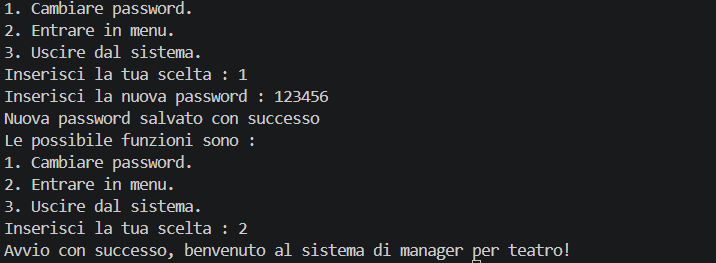
\includegraphics[width=0.85\textwidth]{Test01.png}
    \caption{Schermata di esecuzione del Test T01.}
    \label{fig:test01}
\end{figure}

\subsection{TEST T02}
\begin{listacomp}
    \item \textbf{ID test:} T02
    \item \textbf{Versione:} 0.02
    \item \textbf{Funzionalità testata:} \texttt{int controlladata(char data[])}
    \item \textbf{Input fornito:} stringa di data di lunghezza 11 (nel formato \texttt{gg/mm/aaaa}).
    \item \textbf{Output atteso:} avviso specifico in corrispondenza di ciascun errore di formato o di calendario; valore di ritorno \texttt{-1} in caso di data non valida e \texttt{1} per data corretta.
    \item \textbf{Esito:} Superato.
\end{listacomp}

\begin{lstlisting}[language={}, caption={Output ottenuto durante l'esecuzione del Test T02}]
inserisci la password per entrare in accesso al sistema : 123456
Le possibile funzioni sono : 
1. Cambiare password.
2. Entrare in menu.
3. Uscire dal sistema.
Inserisci la tua scelta : 2
Avvio con successo, benvenuto al sistema di manager per teatro!
inserisci numero massimo di spettacoli da gestire : 12
inserisci numero massimo di clienti da gestire : 12
Le funzionalita' disponibili divisi per categorie sono : 
A. Gestione Spettacoli.
B. Gestione Clienti.
C. Gestione Prenotazioni.
D. Statistiche e Report.
E. Gestioone File.
F. Esci.
Inserisci la tua scelta : a
Le funzionalita' per gestione dei spettacoli sono : 
1. Inserisci nuovo spettacolo.
2. VIsualizza tutti gli spettacoli.
3. Cerca spettacolo per codice.
4. Cerca spettacoli per genere.
5. Spettacoli con posti disponibili.
6. Esci dal menu secondario.
Inserisci la tua scelta : 1
Inserisci codie spettacolo corrispondente : 12
Inserisci titolo dello spettacolo con massimo 100 caratteri : 12
Inserisci genere dello spettacolo con massimo 30 caratteri : 12
Inserisci data dello spettacolo con formato gg/mm/aaaa : 12
Inserisci una data con formato gg/mm/aaaa
Si chiede di inserire una data valida con formato corrispondente segnato
Inserisci data dello spettacolo con formato gg/mm/aaaa : 12/13/2004
Inserisci un mese compreso tra 1 e 12
Si chiede di inserire una data valida con formato corrispondente segnato
Inserisci data dello spettacolo con formato gg/mm/aaaa : 31/11/2004
Nel mese 11 non ha 31 giorni, inserisci una data valida
Si chiede di inserire una data valida con formato corrispondente segnato
Inserisci data dello spettacolo con formato gg/mm/aaaa : 29/02/2003
Nel febbraio del 2003 non ha 29 giorni
Si chiede di inserire una data valida con formato corrispondente segnato
Inserisci data dello spettacolo con formato gg/mm/aaaa : 12 / 12 / 2014
Inserisci una data con formato gg/mm/aaaa
Inserisci data dello spettacolo con formato gg/mm/aaaa : 12/12/2014
Data valida e inserito correttamente
Inserisci posti totali dello spettacolo : 
\end{lstlisting}

\begin{figure}[htbp]
    \centering
    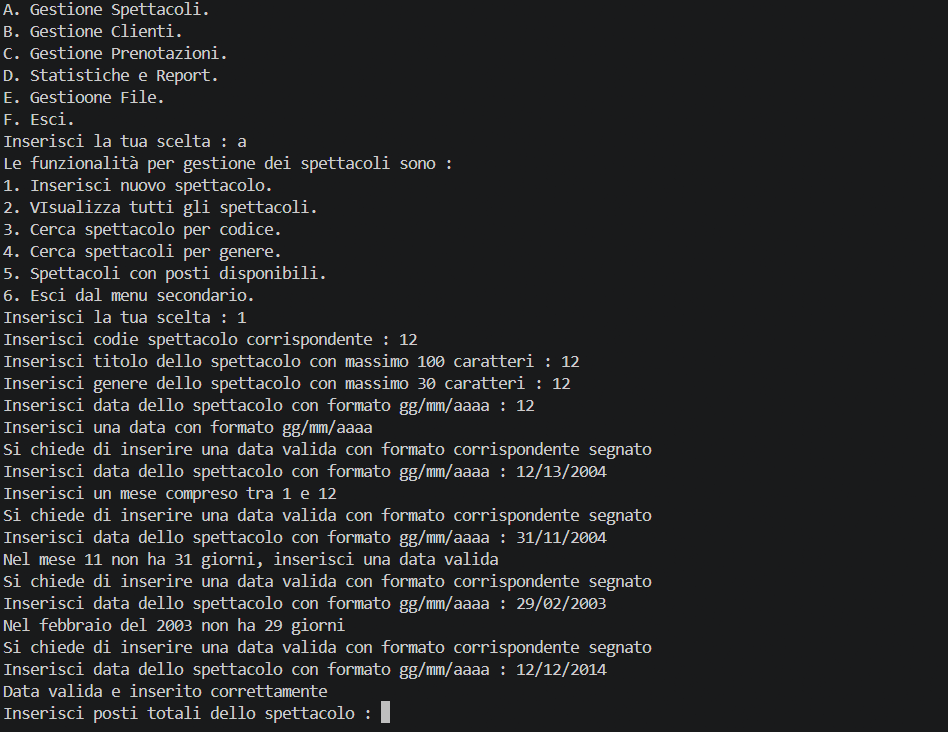
\includegraphics[width=0.85\textwidth]{Test02.png}
    \caption{Schermata di esecuzione del Test T02.}
    \label{fig:test02}
\end{figure}

\subsection{TEST T03}
\begin{listacomp}
    \item \textbf{ID test:} T03
    \item \textbf{Versione:} 0.03 (versione non pubblicata)
    \item \textbf{Funzionalità testata:} \texttt{void inserimentocliente(Cliente *Clienti)}
    \item \textbf{Input fornito:} codice, nome, cognome ed email del cliente.
    \item \textbf{Output atteso:} messaggio di conferma del salvataggio (\texttt{"dati dello cliente salvato correttamente"}).
    \item \textbf{Esito:} Fallito.
    \item \textbf{Motivo:} errore logico nella condizione del ciclo \texttt{while} di verifica dell'email, in cui l'uso dell'operatore \texttt{||} al posto di \texttt{\&\&} ha generato un ciclo infinito con conseguente lettura fuori dai limiti e \emph{Segmentation fault} (\texttt{SIGSEGV}).
\end{listacomp}

\begin{lstlisting}[language={}, caption={Traccia di errore rilevata dal debugger nel Test T03}]
Thread 1 received signal SIGSEGV, Segmentation fault.
0x00007ff767712090 in controllaemail (email=0x5ffd70 "1") at C:\Users\Utente\Desktop\Primo_progetto_parziale\sistema.c:551
551	        return 1;
Execute debugger commands using "-exec <command>", for example "-exec info registers" will list registers in use (when GDB is the debugger)
Kill the program being debugged? (y or n) [answered Y; input not from terminal]
[Inferior 1 (process 18908) killed]
The program 'C:\Users\Utente\Desktop\Primo_progetto_parziale\sistema.exe' has exited with code 0 (0x00000000).
\end{lstlisting}

\begin{figure}[htbp]
    \centering
    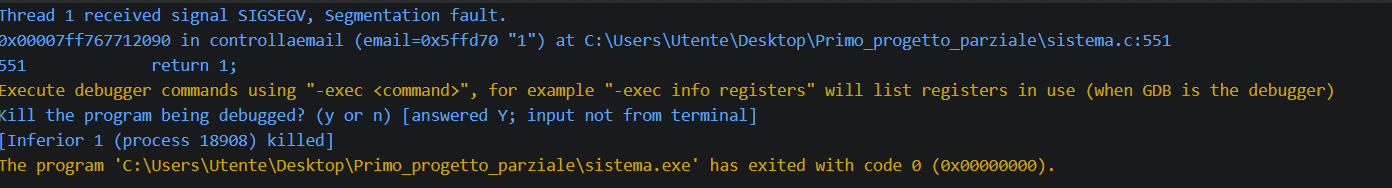
\includegraphics[width=0.85\textwidth]{Test03.png}
    \caption{Schermata di debug relativa al Test T03.}
    \label{fig:test03}
\end{figure}

\subsection{TEST T05}
\begin{listacomp}
    \item \textbf{ID test:} T05
    \item \textbf{Versione:} 0.04 (versione non pubblicata)
    \item \textbf{Funzionalità testata:} Statistiche e report (\texttt{menustat()}).
    \item \textbf{Input fornito:} dati di spettacoli, clienti, prenotazioni e richieste in attesa.
    \item \textbf{Output atteso:} calcolo e visualizzazione dei dati statistici nel formato tabellare previsto.
    \item \textbf{Esito:} Superato.
    \item \textbf{Note:} a seguito del test è stata ridotta la larghezza della colonna dedicata al nome del genere per migliorare l'incolonnamento, ed è stato aggiunto il modificatore di allineamento \texttt{-} sull'intestazione \texttt{Incasso}.
\end{listacomp}

\begin{lstlisting}[language={}, caption={Output ottenuto durante l'esecuzione del Test T05}]
Le funzionalita' disponibili divisi per categorie sono : 
A. Gestione Spettacoli.
B. Gestione Clienti.
C. Gestione Prenotazioni.
D. Statistiche e Report.
E. Gestioone File.
F. Esci.
Inserisci la tua scelta : d
Le funzionalita' per statistiche e report sono : 
1. Statistiche generali.
2. Spettacoli per genere.
3. Top 5 spettacoli per incasso.
4. Esci dal menu secondario.
Inserisci la tua scelta : 1
In cartellone contiene 4 spettacoli
In tutto rimane ancora 198 posti disponibili
In cartellone contiene 2 clienti registrati
In cartellone contiene 3 prenotazione attiva
In cartellone contiene 1 richieste in attesa
Incasso totale e' : 160.00 
Lo spettacolo 01 ha piu' posti prenotati
La media di occupazione e' : 18 %
Le funzionalita' per statistiche e report sono : 
1. Statistiche generali.
2. Spettacoli per genere.
3. Top 5 spettacoli per incasso.
4. Esci dal menu secondario.
Inserisci la tua scelta : 2
Numero di spettacoli presenti divise per genere sono :
Opera                          : 1   spettacoli
Teatro                         : 1   spettacoli
Film                           : 2   spettacoli

/* Dopo ulteriori inserimenti */

Le funzionalita' per statistiche e report sono : 
1. Statistiche generali.
2. Spettacoli per genere.
3. Top 5 spettacoli per incasso.
4. Esci dal menu secondario.
Inserisci la tua scelta : 3
Gli top 5 spettacoli con maggiore incasso sono :
Posizione  Titolo               Genere               Incasso             
0          01                   Opera                            120.00
3          04                   Film                              30.00
1          02                   Teatro                            10.00
2          03                   Film                               0.00
4          05                   Articolo                           0.00
\end{lstlisting}

\begin{figure}[htbp]
    \centering
    \begin{minipage}{0.48\textwidth}
        \centering
        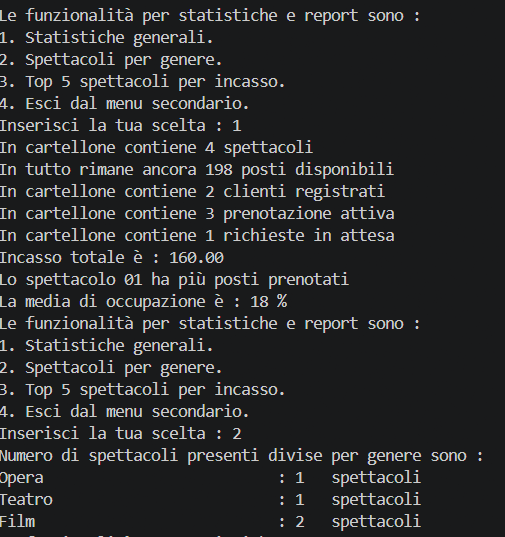
\includegraphics[width=\textwidth]{Test05_1.png}
    \end{minipage}\hfill
    \begin{minipage}{0.48\textwidth}
        \centering
        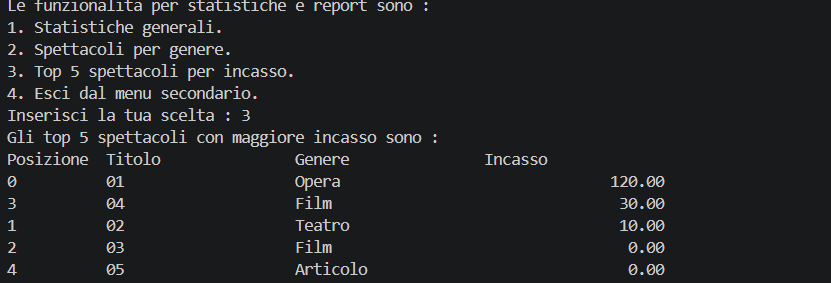
\includegraphics[width=\textwidth]{Test05_2.png}
    \end{minipage}
    \caption{Schermate di esecuzione del Test T05.}
    \label{fig:test05}
\end{figure}

\subsection{TEST T11}
\begin{listacomp}
    \item \textbf{ID test:} T11
    \item \textbf{Versione:} 1.1
    \item \textbf{Funzionalità testata:} inserimento spettacolo con codice duplicato (\texttt{inserimentospettacolo()} / \texttt{controllacodiceSp()}).
    \item \textbf{Input fornito:} dati di uno spettacolo con codice già presente in archivio.
    \item \textbf{Output atteso:} avviso di duplicazione del codice e ritorno alla richiesta di inserimento di un nuovo codice univoco.
    \item \textbf{Esito:} Superato.
\end{listacomp}

\begin{lstlisting}[language={}, caption={Output ottenuto durante l'esecuzione del Test T11}]
inserisci la password per entrare in accesso al sistema : 123456
Le funzionalita' per gestione dei spettacoli sono : 
1. Inserisci nuovo spettacolo.
2. VIsualizza tutti gli spettacoli.
3. Cerca spettacolo per codice.
4. Cerca spettacoli per genere.
5. Spettacoli con posti disponibili.
6. Esci dal menu secondario.
Inserisci la tua scelta : 2
Elenco completo dei spettacoli presenti sono : 
Codice               Titolo               Genere               data                 posti disponibili/posti totali                Prezzo biglietto
0                    0                    0                    12/12/2004                           0/1                                    1.00
Le funzionalita' per gestione dei spettacoli sono : 
1. Inserisci nuovo spettacolo.
2. VIsualizza tutti gli spettacoli.
3. Cerca spettacolo per codice.
4. Cerca spettacoli per genere.
5. Spettacoli con posti disponibili.
6. Esci dal menu secondario.
Inserisci la tua scelta : 1
Inserisci codice spettacolo corrispondente : 0
codice gia' esistente e deve essere univoco, riprova.
Inserisci codice spettacolo corrispondente : 
\end{lstlisting}

\begin{figure}[htbp]
    \centering
    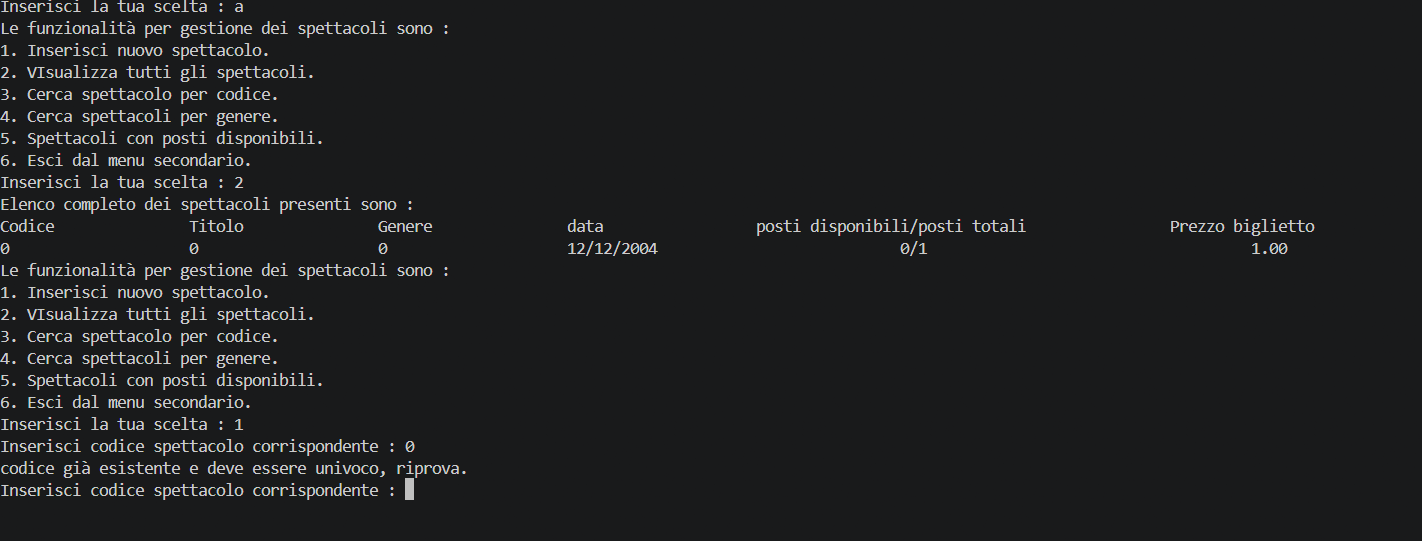
\includegraphics[width=0.85\textwidth]{Test11.png}
    \caption{Schermata di esecuzione del Test T11.}
    \label{fig:test11}
\end{figure}

\subsection{TEST T12}
\begin{listacomp}
    \item \textbf{ID test:} T12
    \item \textbf{Versione:} 1.1
    \item \textbf{Funzionalità testata:} ricerca spettacolo esistente (\texttt{cercacodicespettacolo()}).
    \item \textbf{Input fornito:} codice di uno spettacolo presente in archivio.
    \item \textbf{Output atteso:} stampa tabellare dei dati dello spettacolo corrispondente al codice inserito.
    \item \textbf{Esito:} Superato.
\end{listacomp}

\begin{lstlisting}[language={}, caption={Output ottenuto durante l'esecuzione del Test T12}]
Le funzionalita' per gestione dei spettacoli sono : 
1. Inserisci nuovo spettacolo.
2. VIsualizza tutti gli spettacoli.
3. Cerca spettacolo per codice.
4. Cerca spettacoli per genere.
5. Spettacoli con posti disponibili.
6. Esci dal menu secondario.
Inserisci la tua scelta : 3
Insersci il codice dello spettacolo da cercare : 3
Lo spettacolo corrispondente al codice 3 e' : 
Codice               Titolo               Genere               data                 posti disponibili/posti totali           Prezzo biglietto    
3                    12                   12                   12/12/2004                          19/19                                   2.00
\end{lstlisting}

\begin{figure}[htbp]
    \centering
    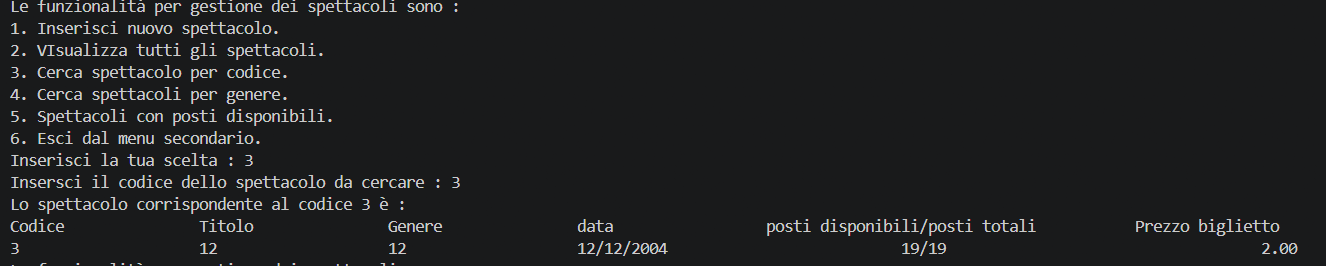
\includegraphics[width=0.85\textwidth]{Test12.png}
    \caption{Schermata di esecuzione del Test T12.}
    \label{fig:test12}
\end{figure}

\subsection{TEST T13}
\begin{listacomp}
    \item \textbf{ID test:} T13
    \item \textbf{Versione:} 1.1
    \item \textbf{Funzionalità testata:} ricerca spettacolo non esistente (\texttt{cercacodicespettacolo()}).
    \item \textbf{Input fornito:} codice di uno spettacolo non presente in archivio.
    \item \textbf{Output atteso:} avviso che nessun spettacolo corrisponde al codice inserito.
    \item \textbf{Esito:} Superato.
\end{listacomp}

\begin{lstlisting}[language={}, caption={Output ottenuto durante l'esecuzione del Test T13}]
Le funzionalita' per gestione dei spettacoli sono : 
1. Inserisci nuovo spettacolo.
2. VIsualizza tutti gli spettacoli.
3. Cerca spettacolo per codice.
4. Cerca spettacoli per genere.
5. Spettacoli con posti disponibili.
6. Esci dal menu secondario.
Inserisci la tua scelta : 3
Insersci il codice dello spettacolo da cercare : 2
il codice inserito non corrisponde ad alcun spettacolo presenti.
\end{lstlisting}

\begin{figure}[htbp]
    \centering
    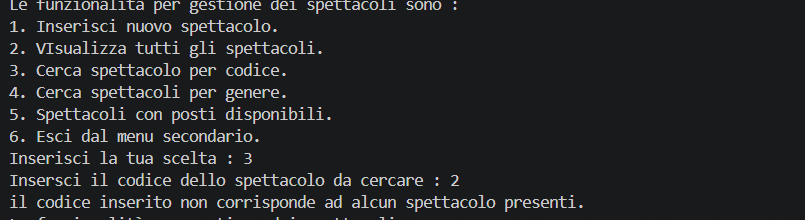
\includegraphics[width=0.85\textwidth]{Test13.png}
    \caption{Schermata di esecuzione del Test T13.}
    \label{fig:test13}
\end{figure}

\subsection{TEST T14}
\begin{listacomp}
    \item \textbf{ID test:} T14
    \item \textbf{Versione:} 1.1
    \item \textbf{Funzionalità testata:} prenotazione con posti disponibili sufficienti (\texttt{registraprenotazione()}).
    \item \textbf{Input fornito:} codice spettacolo, codice cliente, una data valida e un numero di posti valido rientrante nella disponibilità residua.
    \item \textbf{Output atteso:} registrazione della prenotazione con assegnazione automatica del codice univoco e calcolo dell'importo totale.
    \item \textbf{Esito:} Superato.
\end{listacomp}

\begin{lstlisting}[language={}, caption={Output ottenuto durante l'esecuzione del Test T14}]
Inserisci la tua scelta : 1
Inserisci codice spettacole della prenotazione corrispondente : 1
codice inserito corrisponde allo spettaco 12 nella data 12/12/2004 con 17 posti disponibili.
Inserisci codice cliente della prenotazione corrispondente : 0
codice cliente corrisponde al cliente 0 0.
Inserisci numero di posti desiderati : 9
Inserisci data della prenotazione in formato gg/mm/aaaa : 12/12/2004
Data valida e inserito correttamente
I costi totali della prenotazione e' : 18.00.
Per confermare prenotazione inserisci 1, altrimenti 0 : 1
Prenotazione effettuato correttamente.
Ecco gli dati della prenotazione : 
codice prenotazione  codice spettacolo    codice cliente       numero posti         importo totale       data prenotazione   
1                    1                    0                    9                    18.00                12/12/2004          
Le funzionalita' per gestione dei prenotazioni sono : 
\end{lstlisting}

\begin{figure}[htbp]
    \centering
    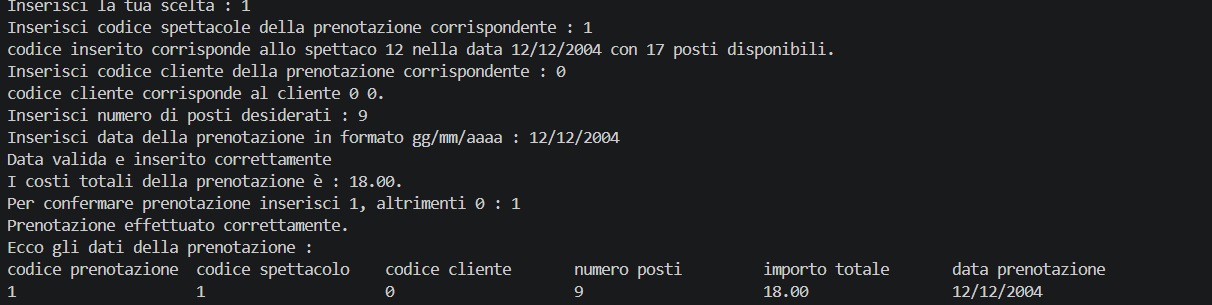
\includegraphics[width=0.85\textwidth]{Test14.png}
    \caption{Schermata di esecuzione del Test T14.}
    \label{fig:test14}
\end{figure}

\subsection{TEST T15}
\begin{listacomp}
    \item \textbf{ID test:} T15
    \item \textbf{Versione:} 1.1
    \item \textbf{Funzionalità testata:} prenotazione con posti disponibili insufficienti e inserimento in lista d'attesa (\texttt{registraprenotazione()}).
    \item \textbf{Input fornito:} codice spettacolo, codice cliente, una data valida e un numero di posti valido ma superiore ai posti disponibili.
    \item \textbf{Output atteso:} segnalazione di posti insufficienti e accodamento della richiesta nella lista d'attesa previa conferma.
    \item \textbf{Esito:} Superato.
\end{listacomp}

\begin{lstlisting}[language={}, caption={Output ottenuto durante l'esecuzione del Test T15}]
Inserisci la tua scelta : 1
Inserisci codice spettacole della prenotazione corrispondente : 1
codice inserito corrisponde allo spettaco 12 nella data 12/12/2004 con 8 posti disponibili.
Inserisci codice cliente della prenotazione corrispondente : 1
codice cliente corrisponde al cliente Mario Rossi.
Inserisci numero di posti desiderati : 9
Inserisci data della prenotazione in formato gg/mm/aaaa : 12/12/2004
Data valida e inserito correttamente
I costi totali della prenotazione e' : 18.00.
Nello spettacolo 12 non ci sono posti sufficienti.
Se desideri aggiungere nella lista d'attesa inserisci 1, altrimenti 0 : 1
dati salvati nella lista di attesa.
\end{lstlisting}

\begin{figure}[htbp]
    \centering
    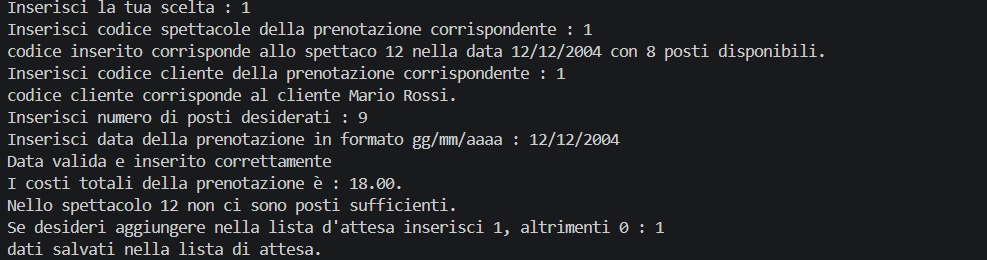
\includegraphics[width=0.85\textwidth]{Test15.png}
    \caption{Schermata di esecuzione del Test T15.}
    \label{fig:test15}
\end{figure}

\subsection{TEST T16}
\begin{listacomp}
    \item \textbf{ID test:} T16
    \item \textbf{Versione:} 1.2
    \item \textbf{Funzionalità testata:} annullamento prenotazione in coda e promozione automatica (\texttt{annullaprenotazione()} / \texttt{converteprenotazione()}).
    \item \textbf{Input fornito:} codice di una prenotazione attiva da annullare.
    \item \textbf{Output atteso:} annullamento della prenotazione e promozione automatica in prenotazione attiva della richiesta compatibile in lista d'attesa.
    \item \textbf{Esito:} Superato.
\end{listacomp}

\begin{lstlisting}[language={}, caption={Output ottenuto durante l'esecuzione del Test T16}]
Le funzionalita' per gestione dei prenotazioni sono : 
1. Registra nuova prenotazione.
2. Annulla prenotazione.
3. Visualizza tutte le prenotazioni.
4. Visualizza prenotazioni di un cliente.
5. Visualizza prenotazioni di uno spettacolo.
6. Visualizza lista d'attesa.
7. Esci dal menu secondario.
Inserisci la tua scelta : 2
Insersci codice di prenotazione per annullazione : 1
Promozione attesa del spettacolo con codice 1 del cliente con codice 2 ad 6 posti
\end{lstlisting}

\begin{figure}[htbp]
    \centering
    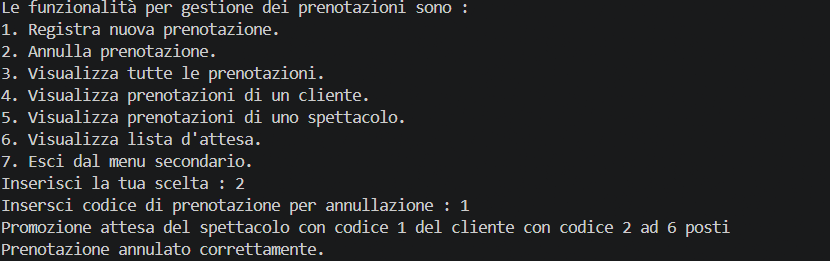
\includegraphics[width=0.85\textwidth]{Test16.png}
    \caption{Schermata di esecuzione del Test T16.}
    \label{fig:test16}
\end{figure}

\section{Test su File}

\subsection{TEST T06}
\begin{listacomp}
    \item \textbf{ID test:} T06
    \item \textbf{Versione:} 0.04 (versione non pubblicata)
    \item \textbf{Funzionalità testata:} \texttt{salvadatabase()}
    \item \textbf{Input fornito:} dati di spettacoli, clienti, prenotazioni e richieste in attesa.
    \item \textbf{Output atteso:} salvataggio corretto degli archivi nei rispettivi file binari (\texttt{.dat}).
    \item \textbf{Esito:} Superato.
\end{listacomp}

\begin{lstlisting}[language={}, caption={Output ottenuto durante l'esecuzione del Test T06}]
Inserisci la tua scelta : e
Le funzionalita' per gestione dei file sono : 
1. Salva database su file binario.
2. Carica database da file binario.
3. Esporta catalogo in formato testo.
4. Esporta report prenotazioni in formato testo.
5. Esci dal menu secondario.
Inserisci la tua scelta : 1
Dati di spettacoli salvati correttamente nel file spettacoli.dat
Dati di Clienti salvati correttamente nel file clienti.dat
Dati nella lista di prenotazioni salvati correttamente nel file prenotazioni.dat
Dati nella lista di attesa salvati correttamente nel file attesa.dat
\end{lstlisting}

\begin{figure}[htbp]
    \centering
    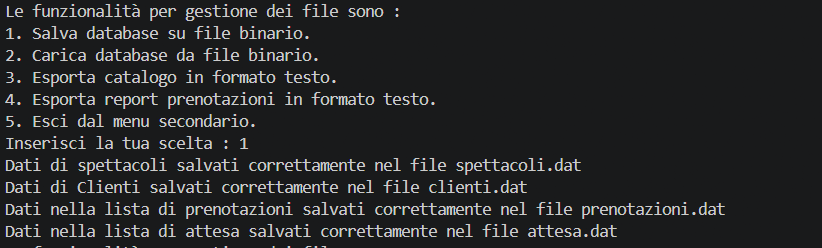
\includegraphics[width=0.85\textwidth]{Test06.png}
    \caption{Schermata di esecuzione del Test T06.}
    \label{fig:test06}
\end{figure}

\subsection{TEST T07}
\begin{listacomp}
    \item \textbf{ID test:} T07
    \item \textbf{Versione:} 0.04 (versione non pubblicata)
    \item \textbf{Funzionalità testata:} \texttt{caricadatabase()}
    \item \textbf{Input fornito:} file binari di archivio (\texttt{.dat}).
    \item \textbf{Output atteso:} caricamento corretto di tutti i file in memoria.
    \item \textbf{Esito:} Fallito.
    \item \textbf{Motivo:} poiché \texttt{Spettacoli} è passato alla funzione come doppio puntatore (\texttt{Spettacolo **}), nella chiamata a \texttt{fread()} è necessario passare \texttt{*Spettacoli} anziché \texttt{Spettacoli}, mentre nella chiamata a \texttt{valutagenere()} occorre dereferenziare correttamente l'elemento tramite \texttt{(*Spettacoli)[i].genere}.
\end{listacomp}

\begin{lstlisting}[language={}, caption={Errori riscontrati durante l'esecuzione del Test T07}]
Segmentation fault per riga : flag = fread(Spettacoli, sizeof(Spettacolo), *num_spettacoli, fp);

Unknown fault per riga : *generi = valutagenere(Spettacoli[i]->genere, *generi);
\end{lstlisting}

\begin{figure}[htbp]
    \centering
    \begin{minipage}{0.48\textwidth}
        \centering
        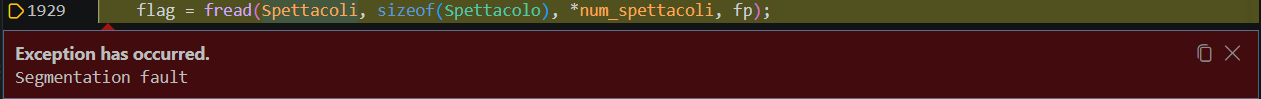
\includegraphics[width=\textwidth]{Test07_1.png}
    \end{minipage}\hfill
    \begin{minipage}{0.48\textwidth}
        \centering
        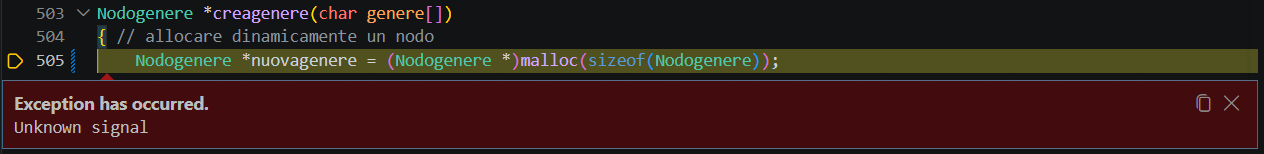
\includegraphics[width=\textwidth]{Test07_2.png}
    \end{minipage}
    \caption{Schermate di errore relative al Test T07.}
    \label{fig:test07}
\end{figure}

\subsection{TEST T08}
\begin{listacomp}
    \item \textbf{ID test:} T08
    \item \textbf{Versione:} 0.04 (versione non pubblicata)
    \item \textbf{Funzionalità testata:} \texttt{caricadatabase()}
    \item \textbf{Input fornito:} file binari di archivio (\texttt{.dat}).
    \item \textbf{Output atteso:} caricamento corretto di tutti i file in memoria.
    \item \textbf{Esito:} Fallito.
    \item \textbf{Motivo:} errato posizionamento delle parentesi nella condizione \texttt{if (controllospazio(*num\_clienti, Maxclienti == -1))}, che confrontava \texttt{Maxclienti} con \texttt{-1} prima di passare il valore alla funzione; inoltre, essendo \texttt{Maxclienti} ancora dichiarato come variabile globale in questa versione, il compilatore non ha segnalato l'anomalia.
\end{listacomp}

\begin{lstlisting}[language={}, caption={Comportamento anomalo rilevato nel Test T08}]
Richiesta di riallocazione per spazio ancora sufficienti.
\end{lstlisting}

\begin{figure}[htbp]
    \centering
    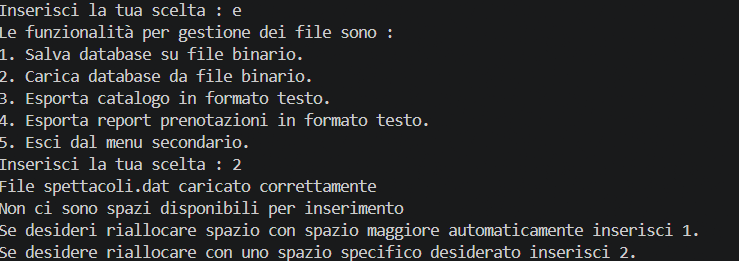
\includegraphics[width=0.85\textwidth]{Test08.png}
    \caption{Schermata di esecuzione del Test T08.}
    \label{fig:test08}
\end{figure}

\subsection{TEST T09}
\begin{listacomp}
    \item \textbf{ID test:} T09
    \item \textbf{Versione:} 0.04 (versione non pubblicata)
    \item \textbf{Funzionalità testata:} \texttt{caricadatabase()}
    \item \textbf{Input fornito:} file binari di archivio (\texttt{.dat}).
    \item \textbf{Output atteso:} caricamento corretto di tutti i file in memoria.
    \item \textbf{Esito:} Fallito.
    \item \textbf{Motivo:} nella riga \texttt{flag = fread(Clienti, sizeof(Spettacolo), *num\_spettacoli, fp);}, copiata dalla sezione degli spettacoli, non erano stati aggiornati né la dimensione del record (\texttt{sizeof(Cliente)}), né il contatore (\texttt{*num\_clienti}), né la dereferenziazione \texttt{*Clienti}, causando il fallimento del successivo controllo di lettura.
\end{listacomp}

\begin{lstlisting}[language={}, caption={Output ottenuto durante l'esecuzione del Test T09}]
Errore operazione sul file
\end{lstlisting}

\begin{figure}[htbp]
    \centering
    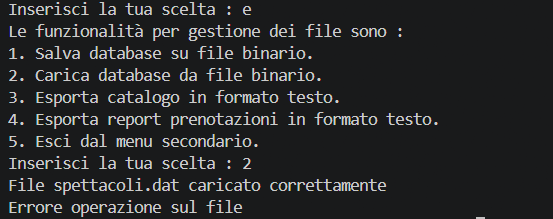
\includegraphics[width=0.85\textwidth]{Test09.png}
    \caption{Schermata di esecuzione del Test T09.}
    \label{fig:test09}
\end{figure}

\subsection{TEST T10}
\begin{listacomp}
    \item \textbf{ID test:} T10
    \item \textbf{Versione:} 0.04 (versione non pubblicata)
    \item \textbf{Funzionalità testata:} \texttt{caricadatabase()}
    \item \textbf{Input fornito:} file binari di archivio (\texttt{.dat}).
    \item \textbf{Output atteso:} caricamento corretto di tutti i file in memoria.
    \item \textbf{Esito:} Superato.
\end{listacomp}

\begin{lstlisting}[language={}, caption={Output ottenuto durante l'esecuzione del Test T10}]
Le funzionalita' per gestione dei file sono : 
1. Salva database su file binario.
2. Carica database da file binario.
3. Esporta catalogo in formato testo.
4. Esporta report prenotazioni in formato testo.
5. Esci dal menu secondario.
Inserisci la tua scelta : 2
File spettacoli.dat caricato correttamente
File clienti.dat caricato correttamente
File prenotazioni.dat caricato correttamente
File attesa.dat caricato correttamente
\end{lstlisting}

\begin{figure}[htbp]
    \centering
    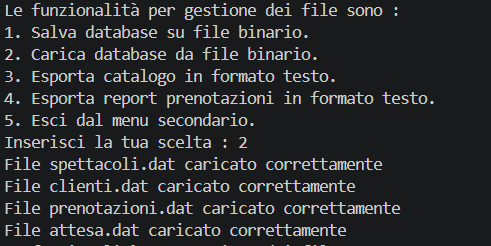
\includegraphics[width=0.85\textwidth]{Test10.png}
    \caption{Schermata di esecuzione del Test T10.}
    \label{fig:test10}
\end{figure}

\subsection{TEST T17}
\begin{listacomp}
    \item \textbf{ID test:} T17
    \item \textbf{Versione:} 1.2
    \item \textbf{Funzionalità testata:} verifica integrità del caricamento dati (\texttt{caricadatabase()}).
    \item \textbf{Input fornito:} file binari di archivio (\texttt{.dat}) precedentemente salvati.
    \item \textbf{Output atteso:} caricamento completo degli archivi e ricostruzione delle liste nell'ordine cronologico corretto.
    \item \textbf{Esito:} Superato.
\end{listacomp}

\begin{lstlisting}[language={}, caption={Output ottenuto durante l'esecuzione del Test T17}]
File spettacoli.dat caricato correttamente
File clienti.dat caricato correttamente
File prenotazioni.dat caricato correttamente
File attesa.dat caricato correttamente
Le funzionalita' per gestione dei file sono : 
1. Salva database su file binario.
2. Carica database da file binario.
3. Esporta catalogo in formato testo.
4. Esporta report prenotazioni in formato testo.
5. Esci dal menu secondario.
Inserisci la tua scelta : 5
Le funzionalita' disponibili divisi per categorie sono : 
A. Gestione Spettacoli.
B. Gestione Clienti.
C. Gestione Prenotazioni.
D. Statistiche e Report.
E. Gestioone File.
F. Esci.
Inserisci la tua scelta : c
Le funzionalita' per gestione dei prenotazioni sono : 
1. Registra nuova prenotazione.
2. Annulla prenotazione.
3. Visualizza tutte le prenotazioni.
4. Visualizza prenotazioni di un cliente.
5. Visualizza prenotazioni di uno spettacolo.
6. Visualizza lista d'attesa.
7. Esci dal menu secondario.
Inserisci la tua scelta : 3
Tutte le prenotazione registrate sono :
codice prenotazione  codice spettacolo    codice cliente       numero posti         importo totale       data prenotazione   
0                    0                    0                    1                    1.00                 12/12/2004          
2                    1                    1                    8                    16.00                12/12/2004          
3                    1                    2                    6                    12.00                12/12/2004      
\end{lstlisting}

\begin{figure}[htbp]
    \centering
    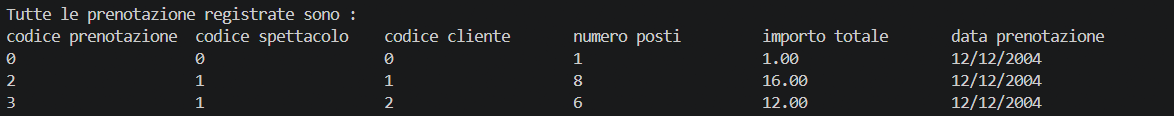
\includegraphics[width=0.85\textwidth]{Test17.png}
    \caption{Schermata di esecuzione del Test T17.}
    \label{fig:test17}
\end{figure}

\subsection{TEST T18}
\begin{listacomp}
    \item \textbf{ID test:} T18
    \item \textbf{Versione:} 1.2
    \item \textbf{Funzionalità testata:} caricamento con file inesistente (\texttt{caricadatabase()}).
    \item \textbf{Input fornito:} selezione dell'opzione di caricamento da file in assenza dei file binari nella cartella di lavoro.
    \item \textbf{Output atteso:} segnalazione controllata dell'errore di apertura del file senza arresto anomalo del programma.
    \item \textbf{Esito:} Superato.
\end{listacomp}

\begin{lstlisting}[language={}, caption={Output ottenuto durante l'esecuzione del Test T18}]
Inserisci la tua scelta : 2
Caricando dati dal file, si perde tutti i dati presenti nell'array, sei sicura di continuare?
Per conferma inserisci 1, altrimenti un qualsiasi altro numero intero : 1
Errore apertura file spettacoli.dat
Si e' verificato un errore per caricare dati dal file
\end{lstlisting}

\begin{figure}[htbp]
    \centering
    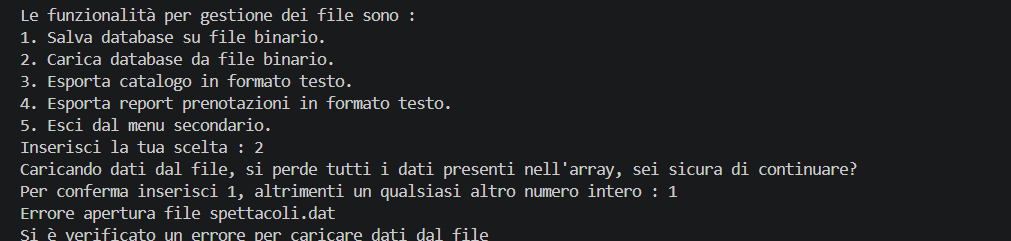
\includegraphics[width=0.85\textwidth]{Test18.png}
    \caption{Schermata di esecuzione del Test T18.}
    \label{fig:test18}
\end{figure}

\subsection{TEST T19}
\begin{listacomp}
    \item \textbf{ID test:} T19
    \item \textbf{Versione:} 1.2
    \item \textbf{Funzionalità testata:} esportazione dei file di testo (\texttt{esportacatalogo()}).
    \item \textbf{Input fornito:} elenco degli spettacoli presenti in memoria.
    \item \textbf{Output atteso:} scrittura corretta dei dati formattati nel file testuale \texttt{catalogo.txt}.
    \item \textbf{Esito:} Superato.
\end{listacomp}

\begin{lstlisting}[language={}, caption={Output ottenuto durante l'esecuzione del Test T19}]
Le funzionalita' per gestione dei file sono : 
1. Salva database su file binario.
2. Carica database da file binario.
3. Esporta catalogo in formato testo.
4. Esporta report prenotazioni in formato testo.
5. Esci dal menu secondario.
Inserisci la tua scelta : 3
Dati dei spettacoli scritti correttamente in catalogo.txt
\end{lstlisting}

\begin{figure}[htbp]
    \centering
    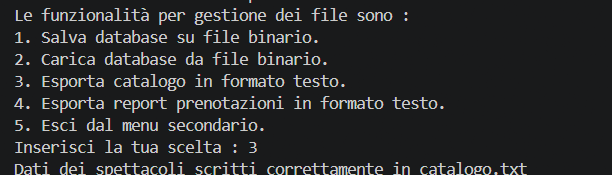
\includegraphics[width=0.85\textwidth]{Test19.png}
    \caption{Schermata di esecuzione del Test T19.}
    \label{fig:test19}
\end{figure}

\chapter{Manuale Utente}

Il presente manuale illustra le procedure operative per l'utilizzo del sistema gestionale per il teatro, guidando l'utente dall'autenticazione iniziale fino alla gestione degli archivi e alla generazione dei report.

\section{Accesso al sistema e inizializzazione}
All'avvio dell'applicazione viene eseguita la procedura di autenticazione per consentire l'accesso esclusivamente al personale autorizzato:
\begin{listacomp}
    \item \textbf{Inserimento della password:} digitare la password numerica richiesta a schermo e premere \texttt{Invio}. Al primo avvio del programma (in assenza del file \texttt{password.dat}), la password predefinita è \texttt{123456}.
    \item \textbf{Gestione dell'errore di accesso:} qualora la password inserita non sia corretta, il sistema consente di ripetere il tentativo digitando \texttt{1}, oppure di chiudere immediatamente il programma inserendo qualsiasi altro numero intero.
    \item \textbf{Menu preliminare di accesso:} superata la verifica, vengono proposte tre opzioni:
    \begin{listacomp}
        \item \texttt{1. Cambiare password:} permette di impostare una nuova password numerica (diversa da quella precedente), che viene salvata in formato codificato nel file \texttt{password.dat} per gli accessi successivi.
        \item \texttt{2. Entrare in menu:} avvia la sessione operativa vera e propria.
        \item \texttt{3. Uscire dal sistema:} termina l'esecuzione del programma.
    \end{listacomp}
    \item \textbf{Configurazione delle capacità iniziali:} subito dopo aver selezionato l'opzione \texttt{2}, il sistema richiede di inserire due numeri interi strettamente positivi per definire la capacità iniziale degli archivi in memoria dedicati agli spettacoli e ai clienti. Tale limite può comunque essere ampliato dinamicamente durante l'utilizzo qualora si superi la capienza impostata.
\end{listacomp}

\section{Struttura del menu principale e delle opzioni}
Terminata la fase iniziale, l'utente accede al menu principale, organizzato in sei categorie selezionabili digitando la lettera corrispondente (maiuscola o minuscola):
\begin{listacomp}
    \item \textbf{\texttt{A} -- Gestione Spettacoli:} consente di inserire nuovi spettacoli in cartellone (\texttt{1}), visualizzare l'elenco completo (\texttt{2}), ricercare uno spettacolo per codice (\texttt{3}) o per genere (\texttt{4}), visualizzare gli spettacoli con posti ancora disponibili ordinati cronologicamente (\texttt{5}) e tornare al menu principale (\texttt{6}).
    \item \textbf{\texttt{B} -- Gestione Clienti:} permette di registrare un nuovo cliente (\texttt{1}), visualizzare l'anagrafica completa (\texttt{2}), cercare un cliente tramite codice identificativo (\texttt{3}) e tornare al menu principale (\texttt{4}).
    \item \textbf{\texttt{C} -- Gestione Prenotazioni:} raccoglie le funzioni per registrare una nuova prenotazione (\texttt{1}), annullare una prenotazione esistente (\texttt{2}), visualizzare tutte le prenotazioni (\texttt{3}), filtrarle per singolo cliente (\texttt{4}) o per singolo spettacolo (\texttt{5}), consultare la lista d'attesa (\texttt{6}) e uscire dal sottomenu (\texttt{7}).
    \item \textbf{\texttt{D} -- Statistiche e Report:} fornisce il riepilogo delle statistiche generali (\texttt{1}), la distribuzione degli spettacoli per genere (\texttt{2}), la classifica dei primi 5 spettacoli per incasso (\texttt{3}) e il ritorno al menu principale (\texttt{4}).
    \item \textbf{\texttt{E} -- Gestione File:} permette di salvare il database su file binari (\texttt{1}), caricare un database precedentemente salvato (\texttt{2}), esportare il catalogo spettacoli in formato testo (\texttt{3}), esportare il report delle prenotazioni in formato testo (\texttt{4}) e tornare al menu principale (\texttt{5}).
    \item \textbf{\texttt{F} -- Esci:} avvia la procedura di chiusura controllata, avvisando che i dati non salvati andranno perduti e chiedendo se uscire direttamente (\texttt{1}), uscire salvando automaticamente i dati su file binari (\texttt{2}) oppure annullare e tornare al menu principale (\texttt{3}).
\end{listacomp}

\section{Come aggiungere uno spettacolo}
Per inserire un nuovo spettacolo in cartellone, selezionare l'opzione \texttt{A} dal menu principale e successivamente l'opzione \texttt{1}:
\begin{listacomp}
    \item \textbf{Eventuale espansione dello spazio:} se l'array degli spettacoli ha raggiunto la capienza massima, il sistema propone di raddoppiare automaticamente lo spazio (\texttt{1}) o di indicare manualmente una nuova capacità (\texttt{2}).
    \item \textbf{Compilazione dei campi richiesti:} inserire in sequenza:
    \begin{listacomp}
        \item \emph{Codice spettacolo:} un numero intero univoco non ancora assegnato ad altri spettacoli.
        \item \emph{Titolo e Genere:} stringhe di testo (rispettivamente fino a 100 e 30 caratteri).
        \item \emph{Data dello spettacolo:} nel formato tassativo \texttt{gg/mm/aaaa} (con anno compreso tra \texttt{2000} e \texttt{2100} e controllo sulla validità dei giorni del mese).
        \item \emph{Posti totali e Prezzo biglietto:} un numero intero strettamente positivo per la capienza della sala (i posti disponibili vengono inizializzati automaticamente allo stesso valore) e un numero positivo per il costo del singolo biglietto.
    \end{listacomp}
    \item \textbf{Conferma finale:} il programma mostra una tabella riepilogativa con i dati appena digitati; inserire \texttt{1} per confermare e salvare lo spettacolo in memoria, oppure \texttt{0} per ripetere l'inserimento.
\end{listacomp}

\section{Come registrare una prenotazione}
Prima di effettuare una prenotazione è necessario che lo spettacolo e il cliente siano già presenti nei rispettivi archivi. Dal menu principale, selezionare \texttt{C} e poi \texttt{1}:
\begin{listacomp}
    \item \textbf{Identificazione di spettacolo e cliente:} digitare il codice dello spettacolo e il codice del cliente. Il sistema verifica l'esistenza di entrambi e mostra a schermo il titolo dello spettacolo con i posti attualmente disponibili e il nominativo del cliente.
    \item \textbf{Quantità e data:} inserire il numero di posti desiderati (compreso tra \texttt{1} e \texttt{10}) e la data della prenotazione nel formato \texttt{gg/mm/aaaa}. Il programma calcola e visualizza automaticamente l'importo totale da pagare.
    \item \textbf{Esito in base alla disponibilità:}
    \begin{listacomp}
        \item \emph{Posti disponibili sufficienti:} digitare \texttt{1} per confermare la prenotazione (purché il cliente non sia già in lista d'attesa per lo stesso spettacolo). Il sistema assegna un codice prenotazione univoco, scala i posti disponibili dello spettacolo e mostra il riepilogo dell'operazione.
        \item \emph{Posti disponibili insufficienti:} il sistema avvisa che la capienza residua non soddisfa la richiesta e chiede se inserire il cliente nella lista d'attesa (\texttt{1} per accodare la richiesta in ordine cronologico, \texttt{0} per annullare).
    \end{listacomp}
\end{listacomp}

\section{Come annullare una prenotazione}
Per cancellare una prenotazione attiva e liberare i relativi biglietti, accedere al menu prenotazioni (\texttt{C}) e selezionare l'opzione \texttt{2}:
\begin{listacomp}
    \item \textbf{Inserimento del codice:} digitare il \texttt{codice prenotazione} da annullare (consultabile preventivamente tramite l'opzione \texttt{3}, \texttt{4} o \texttt{5} dello stesso menu).
    \item \textbf{Aggiornamento dei posti e promozione dalla lista d'attesa:} se il codice corrisponde a una prenotazione esistente, questa viene eliminata e i relativi posti vengono riaccreditati allo spettacolo. Contestualmente, il sistema scorre automaticamente la lista d'attesa in ordine di arrivo (FIFO): se trova richieste per lo stesso spettacolo compatibili con i nuovi posti disponibili, le converte in prenotazioni confermate assegnando loro un nuovo codice univoco.
\end{listacomp}

\section{Come generare statistiche e report}
Per consultare gli indicatori sull'andamento del teatro, selezionare l'opzione \texttt{D} dal menu principale e scegliere una delle tre visualizzazioni disponibili:
\begin{listacomp}
    \item \textbf{\texttt{1. Statistiche generali}:} mostra in un unico prospetto il numero totale di spettacoli in cartellone, i posti ancora disponibili complessivi, il totale dei clienti registrati, il numero di prenotazioni attive e di richieste in attesa, l'incasso totale accumulato, il titolo dello spettacolo con il maggior numero di biglietti venduti e la percentuale media di occupazione delle sale.
    \item \textbf{\texttt{2. Spettacoli per genere}:} elenca tutti i generi teatrali inseriti accompagnati dal numero di spettacoli appartenenti a ciascuna categoria.
    \item \textbf{\texttt{3. Top 5 spettacoli per incasso}:} visualizza una classifica tabellare dei primi 5 spettacoli ordinati in modo decrescente in base all'incasso generato.
\end{listacomp}

\section{Come salvare e caricare i file}
Poiché i dati gestiti durante la sessione risiedono nella memoria centrale volatile, è fondamentale salvarli su disco prima di chiudere il programma. Dal menu principale, selezionare \texttt{E}:
\begin{listacomp}
    \item \textbf{Salvataggio del database (\texttt{1. Salva database su file binario}):} esporta lo stato corrente di tutti gli archivi in quattro file binari nella cartella del programma (\texttt{spettacoli.dat}, \texttt{clienti.dat}, \texttt{prenotazioni.dat} e \texttt{attesa.dat}). La stessa operazione può essere eseguita automaticamente in chiusura scegliendo \texttt{F} e poi \texttt{2}.
    \item \textbf{Caricamento del database (\texttt{2. Carica database da file binario}):} ripristina in memoria i dati salvati nei quattro file \texttt{.dat}. Poiché l'operazione sovrascrive completamente i dati attualmente presenti in memoria, il sistema richiede una conferma esplicita digitando \texttt{1} prima di procedere.
    \item \textbf{Esportazione in formato testo (\texttt{3} e \texttt{4}):} per consultare o stampare i dati al di fuori del programma, l'opzione \texttt{3} genera il file \texttt{catalogo.txt} con l'elenco formattato di tutti gli spettacoli, mentre l'opzione \texttt{4} crea il file \texttt{report\_prenotazioni.txt} contenente il dettaglio di tutte le prenotazioni attive abbinate ai nominativi dei clienti e al riepilogo dell'incasso complessivo.
\end{listacomp}

\chapter{Conclusione}

\section{Obiettivi raggiunti}
Lo sviluppo di questo progetto ha permesso di consolidare in modo approfondito gli argomenti affrontati durante il corso. A differenza dei brevi esercizi svolti a lezione, la realizzazione di un sistema gestionale completo fa emergere numerose problematiche pratiche e casi limite che si manifestano soltanto integrando tra loro strutture dati composte (\texttt{struct}), allocazione dinamica della memoria, gestione dei puntatori sulle liste concatenate e operazioni di lettura e scrittura su file.

\section{Difficoltà incontrate}
Durante la progettazione e l'implementazione del codice sono emerse diverse criticità tecniche, risolte progressivamente attraverso scelte mirate:
\begin{listacomp}
    \item \textbf{Validazione delle date:} inizialmente si era tentato di verificare la correttezza delle date confrontando direttamente i singoli caratteri (\texttt{char}), finendo però per trascurare casistiche fondamentali come gli anni bisestili o la distinzione tra mesi di 30 e 31 giorni. In fase di sviluppo si è quindi compreso che, analizzando la stringa cifra per cifra, è possibile ricostruire i corrispondenti valori interi (tramite \texttt{scanstring()}), rendendo i controlli di calendario e i confronti cronologici molto più semplici e affidabili.
    \item \textbf{Gestione dinamica dei generi:} non potendo conoscere a priori quali generi teatrali verranno inseriti dall'utente, non è possibile predisporre confronti fissi per ciascuna categoria. Per questo motivo, già in fase di progettazione, si è scelto di introdurre una lista concatenata dedicata (\texttt{Nodogenere}): in questo modo i generi vengono censiti e conteggiati dinamicamente a ogni inserimento di uno spettacolo, riducendo il calcolo delle statistiche a un semplice scorrimento della lista.
    \item \textbf{Sostituzione delle variabili globali con puntatori e doppi puntatori:} la necessità di aggiornare in più funzioni i contatori degli elementi presenti (come \texttt{num\_spettacoli}) e le capacità massime modificate durante la \texttt{realloc()} (come \texttt{Maxclienti}) aveva inizialmente portato a dichiarare tali contatori come variabili globali nelle prime versioni del programma. Un problema analogo si è presentato sulle liste concatenate: durante l'annullamento di una prenotazione occorre aggiornare contemporaneamente sia la lista delle prenotazioni sia la lista d'attesa, ma l'istruzione \texttt{return} consente di restituire un solo puntatore, facendo perdere le modifiche apportate alla seconda lista. Seguendo il suggerimento del docente di adottare i doppi puntatori (\texttt{**}) per le liste, è stato revisionato anche il resto del codice eliminando le variabili globali e passando i contatori per indirizzo. Sebbene ciò abbia reso le firme delle funzioni più articolate per l'elevato numero di parametri, questa scelta ha permesso di individuare un bug logico legato a \texttt{Maxclienti} che prima sfuggiva sia al compilatore sia all'esecuzione proprio a causa della visibilità globale della variabile.
\end{listacomp}

\section{Possibili miglioramenti futuri}
Nonostante il sistema soddisfi tutti i requisiti richiesti, si individuano alcuni possibili margini di miglioramento:
\begin{listacomp}
    \item \textbf{Ricerca per genere insensibile alle maiuscole:} nella funzione di ricerca degli spettacoli per genere viene impiegata \texttt{strcmp()} per rispettare le specifiche assegnate, rendendo però il confronto \emph{case-sensitive}. Sostituendola con \texttt{strcasecmp()} (già utilizzata nella gestione della lista statistica \texttt{Nodogenere}), la ricerca risulterebbe più flessibile per l'utente.
    \item \textbf{Uscita anticipata dai cicli di inserimento:} attualmente, una volta avviato un inserimento (ad esempio di un nuovo spettacolo), il programma rimane nei cicli di validazione finché non vengono forniti tutti i dati corretti, senza possibilità di annullare l'operazione a metà. L'aggiunta di una richiesta di uscita a ogni passaggio di errore risolverebbe il limite, ma è stata evitata poiché avrebbe appesantito eccessivamente la struttura del codice in tutte le funzionalità.
    \item \textbf{Salvataggio e caricamento separati per singolo file:} l'implementazione attuale gestisce i quattro file binari in modo unitario. Sebbene sia ipotizzabile suddividere la persistenza in quattro funzioni indipendenti per operare su un singolo archivio alla volta, si è preferito mantenere la gestione sincronizzata poiché i dati sono strettamente interdipendenti: una prenotazione richiede infatti che i codici di spettacolo e cliente esistano negli array in memoria, mentre il caricamento isolato della lista d'attesa potrebbe lasciare richieste non promosse in presenza di posti liberi se non interviene un annullamento a sbloccarle.
\end{listacomp}

\section{Considerazioni personali sull'esperienza}
Lo sviluppo del progetto ha evidenziato quanto sia importante attenersi rigorosamente ai vincoli progettuali fissati: tali specifiche rispondono a obiettivi didattici precisi, anche quando alcune funzionalità potrebbero essere implementate più rapidamente con soluzioni alternative (ad esempio aggiungendo un campo dedicato all'incasso direttamente nella struttura \texttt{Spettacolo} per semplificare l'ordinamento). È inoltre emerso come la parte realmente centrale dello sviluppo risieda nella progettazione logica e nella scelta delle strutture dati: una volta delineata con chiarezza l'architettura, la stesura del codice diventa un'attività prevalentemente meccanica.

Sul fronte del \emph{debugging}, l'aspetto più complesso si è rivelato l'individuazione della causa degli errori: come riscontrato durante i test, un semplice refuso di una lettera tra il prototipo e l'implementazione di una funzione impedisce la compilazione senza che l'editor segnali immediatamente il punto esatto all'interno di oltre 2.000 righe di codice. In questo contesto l'utilizzo di un repository su GitHub si è dimostrato fondamentale, consentendo di confrontare le modifiche rispetto alle versioni precedenti e di sviluppare nuove funzionalità su \emph{branch} separati prima di integrarle nella versione principale. Infine, per quanto riguarda la stesura della relazione tecnica, la sezione di progettazione è risultata particolarmente estesa poiché richiede di richiamare in dettaglio numerosi concetti teorici già trattati nelle dispense del corso.

\end{document}
